\documentclass[]{article}
\usepackage{lmodern}
\usepackage{amssymb,amsmath}
\usepackage{ifxetex,ifluatex}
\usepackage{fixltx2e} % provides \textsubscript
\ifnum 0\ifxetex 1\fi\ifluatex 1\fi=0 % if pdftex
  \usepackage[T1]{fontenc}
  \usepackage[utf8]{inputenc}
\else % if luatex or xelatex
  \ifxetex
    \usepackage{mathspec}
  \else
    \usepackage{fontspec}
  \fi
  \defaultfontfeatures{Ligatures=TeX,Scale=MatchLowercase}
\fi
% use upquote if available, for straight quotes in verbatim environments
\IfFileExists{upquote.sty}{\usepackage{upquote}}{}
% use microtype if available
\IfFileExists{microtype.sty}{%
\usepackage{microtype}
\UseMicrotypeSet[protrusion]{basicmath} % disable protrusion for tt fonts
}{}
\usepackage[margin=1in]{geometry}
\usepackage{hyperref}
\hypersetup{unicode=true,
            pdftitle={Processing, cleaning and saving NZ GREEN Grid project 1 minute electricity consumption data},
            pdfauthor={Ben Anderson (b.anderson@soton.ac.uk, @dataknut)},
            pdfborder={0 0 0},
            breaklinks=true}
\urlstyle{same}  % don't use monospace font for urls
\usepackage{color}
\usepackage{fancyvrb}
\newcommand{\VerbBar}{|}
\newcommand{\VERB}{\Verb[commandchars=\\\{\}]}
\DefineVerbatimEnvironment{Highlighting}{Verbatim}{commandchars=\\\{\}}
% Add ',fontsize=\small' for more characters per line
\usepackage{framed}
\definecolor{shadecolor}{RGB}{248,248,248}
\newenvironment{Shaded}{\begin{snugshade}}{\end{snugshade}}
\newcommand{\KeywordTok}[1]{\textcolor[rgb]{0.13,0.29,0.53}{\textbf{#1}}}
\newcommand{\DataTypeTok}[1]{\textcolor[rgb]{0.13,0.29,0.53}{#1}}
\newcommand{\DecValTok}[1]{\textcolor[rgb]{0.00,0.00,0.81}{#1}}
\newcommand{\BaseNTok}[1]{\textcolor[rgb]{0.00,0.00,0.81}{#1}}
\newcommand{\FloatTok}[1]{\textcolor[rgb]{0.00,0.00,0.81}{#1}}
\newcommand{\ConstantTok}[1]{\textcolor[rgb]{0.00,0.00,0.00}{#1}}
\newcommand{\CharTok}[1]{\textcolor[rgb]{0.31,0.60,0.02}{#1}}
\newcommand{\SpecialCharTok}[1]{\textcolor[rgb]{0.00,0.00,0.00}{#1}}
\newcommand{\StringTok}[1]{\textcolor[rgb]{0.31,0.60,0.02}{#1}}
\newcommand{\VerbatimStringTok}[1]{\textcolor[rgb]{0.31,0.60,0.02}{#1}}
\newcommand{\SpecialStringTok}[1]{\textcolor[rgb]{0.31,0.60,0.02}{#1}}
\newcommand{\ImportTok}[1]{#1}
\newcommand{\CommentTok}[1]{\textcolor[rgb]{0.56,0.35,0.01}{\textit{#1}}}
\newcommand{\DocumentationTok}[1]{\textcolor[rgb]{0.56,0.35,0.01}{\textbf{\textit{#1}}}}
\newcommand{\AnnotationTok}[1]{\textcolor[rgb]{0.56,0.35,0.01}{\textbf{\textit{#1}}}}
\newcommand{\CommentVarTok}[1]{\textcolor[rgb]{0.56,0.35,0.01}{\textbf{\textit{#1}}}}
\newcommand{\OtherTok}[1]{\textcolor[rgb]{0.56,0.35,0.01}{#1}}
\newcommand{\FunctionTok}[1]{\textcolor[rgb]{0.00,0.00,0.00}{#1}}
\newcommand{\VariableTok}[1]{\textcolor[rgb]{0.00,0.00,0.00}{#1}}
\newcommand{\ControlFlowTok}[1]{\textcolor[rgb]{0.13,0.29,0.53}{\textbf{#1}}}
\newcommand{\OperatorTok}[1]{\textcolor[rgb]{0.81,0.36,0.00}{\textbf{#1}}}
\newcommand{\BuiltInTok}[1]{#1}
\newcommand{\ExtensionTok}[1]{#1}
\newcommand{\PreprocessorTok}[1]{\textcolor[rgb]{0.56,0.35,0.01}{\textit{#1}}}
\newcommand{\AttributeTok}[1]{\textcolor[rgb]{0.77,0.63,0.00}{#1}}
\newcommand{\RegionMarkerTok}[1]{#1}
\newcommand{\InformationTok}[1]{\textcolor[rgb]{0.56,0.35,0.01}{\textbf{\textit{#1}}}}
\newcommand{\WarningTok}[1]{\textcolor[rgb]{0.56,0.35,0.01}{\textbf{\textit{#1}}}}
\newcommand{\AlertTok}[1]{\textcolor[rgb]{0.94,0.16,0.16}{#1}}
\newcommand{\ErrorTok}[1]{\textcolor[rgb]{0.64,0.00,0.00}{\textbf{#1}}}
\newcommand{\NormalTok}[1]{#1}
\usepackage{longtable,booktabs}
\usepackage{graphicx,grffile}
\makeatletter
\def\maxwidth{\ifdim\Gin@nat@width>\linewidth\linewidth\else\Gin@nat@width\fi}
\def\maxheight{\ifdim\Gin@nat@height>\textheight\textheight\else\Gin@nat@height\fi}
\makeatother
% Scale images if necessary, so that they will not overflow the page
% margins by default, and it is still possible to overwrite the defaults
% using explicit options in \includegraphics[width, height, ...]{}
\setkeys{Gin}{width=\maxwidth,height=\maxheight,keepaspectratio}
\IfFileExists{parskip.sty}{%
\usepackage{parskip}
}{% else
\setlength{\parindent}{0pt}
\setlength{\parskip}{6pt plus 2pt minus 1pt}
}
\setlength{\emergencystretch}{3em}  % prevent overfull lines
\providecommand{\tightlist}{%
  \setlength{\itemsep}{0pt}\setlength{\parskip}{0pt}}
\setcounter{secnumdepth}{5}
% Redefines (sub)paragraphs to behave more like sections
\ifx\paragraph\undefined\else
\let\oldparagraph\paragraph
\renewcommand{\paragraph}[1]{\oldparagraph{#1}\mbox{}}
\fi
\ifx\subparagraph\undefined\else
\let\oldsubparagraph\subparagraph
\renewcommand{\subparagraph}[1]{\oldsubparagraph{#1}\mbox{}}
\fi

%%% Use protect on footnotes to avoid problems with footnotes in titles
\let\rmarkdownfootnote\footnote%
\def\footnote{\protect\rmarkdownfootnote}

%%% Change title format to be more compact
\usepackage{titling}

% Create subtitle command for use in maketitle
\newcommand{\subtitle}[1]{
  \posttitle{
    \begin{center}\large#1\end{center}
    }
}

\setlength{\droptitle}{-2em}
  \title{Processing, cleaning and saving NZ GREEN Grid project 1 minute
electricity consumption data}
  \pretitle{\vspace{\droptitle}\centering\huge}
  \posttitle{\par}
  \author{Ben Anderson
(\href{mailto:b.anderson@soton.ac.uk}{\nolinkurl{b.anderson@soton.ac.uk}},
\texttt{@dataknut})}
  \preauthor{\centering\large\emph}
  \postauthor{\par}
  \predate{\centering\large\emph}
  \postdate{\par}
  \date{Last run at: 2018-05-07 12:51:59}


\begin{document}
\maketitle

{
\setcounter{tocdepth}{2}
\tableofcontents
}
\newpage

\section{Citation}\label{citation}

If you wish to use any of the material from this report please cite as:

\begin{itemize}
\tightlist
\item
  Anderson, B. (2018) Processing, cleaning and saving NZ GREEN Grid
  project 1 minute electricity consumption data, University of Otago:
  Dunedin, NZ.
\end{itemize}

\newpage

\section{Introduction}\label{introduction}

Report circulation:

\begin{itemize}
\tightlist
\item
  Restricted to:
  \href{https://www.otago.ac.nz/centre-sustainability/research/energy/otago050285.html}{NZ
  GREEn Grid} project partners and contractors.
\end{itemize}

\subsection{Purpose}\label{purpose}

This report is intended to:

\begin{itemize}
\tightlist
\item
  load and clean the project electricity consumption data (Grid Spy)
\item
  save the cleaned data out as a single file per household
\item
  produce summary data quality statistics
\end{itemize}

\subsection{Requirements:}\label{requirements}

\begin{itemize}
\tightlist
\item
  grid spy 1 minute data downloads
\end{itemize}

\subsection{History}\label{history}

Generally tracked via our git.soton
\href{https://git.soton.ac.uk/ba1e12/nzGREENGrid}{repo}.

\subsection{Support}\label{support}

This work was supported by:

\begin{itemize}
\tightlist
\item
  The \href{https://www.otago.ac.nz/}{University of Otago}
\item
  The New Zealand \href{http://www.mbie.govt.nz/}{Ministry of Business,
  Innovation and Employment (MBIE)}
\item
  \href{http://www.energy.soton.ac.uk/tag/spatialec/}{SPATIALEC} - a
  \href{http://ec.europa.eu/research/mariecurieactions/about-msca/actions/if/index_en.htm}{Marie
  Skłodowska-Curie Global Fellowship} based at the University of Otago's
  \href{http://www.otago.ac.nz/centre-sustainability/staff/otago673896.html}{Centre
  for Sustainability} (2017-2019) \& the University of Southampton's
  Sustainable Energy Research Group (2019-202).
\end{itemize}

This work uis (c) 2018 the University of Southampton.

\section{Obtain listing of files}\label{obtain-listing-of-files}

In this section we generate a listing of all 1 minute data files that we
have received. If we are running over the complete dataset then we will
be using data from:

\begin{itemize}
\tightlist
\item
  /hum-csafe/Research Projects/GREEN Grid/\_RAW DATA/GridSpyData/
\end{itemize}

In this run we are using data from:

\begin{itemize}
\tightlist
\item
  /Volumes/hum-csafe/Research Projects/GREEN Grid/\_RAW
  DATA/GridSpyData/
\end{itemize}

If these do not match then this may be a test run.

\begin{Shaded}
\begin{Highlighting}[]
\KeywordTok{print}\NormalTok{(}\KeywordTok{paste0}\NormalTok{(}\StringTok{"Looking for 1 minute data using pattern = "}\NormalTok{, pattern1Min, }\StringTok{" in "}\NormalTok{, fpath, }\StringTok{" - could take a while..."}\NormalTok{))}
\end{Highlighting}
\end{Shaded}

\begin{verbatim}
## [1] "Looking for 1 minute data using pattern = *at1.csv$ in /Volumes/hum-csafe/Research Projects/GREEN Grid/_RAW DATA/GridSpyData/ - could take a while..."
\end{verbatim}

\begin{Shaded}
\begin{Highlighting}[]
\KeywordTok{system.time}\NormalTok{(fListCompleteDT <-}\StringTok{ }\KeywordTok{as.data.table}\NormalTok{(}\KeywordTok{list.files}\NormalTok{(}\DataTypeTok{path =}\NormalTok{ fpath, }\DataTypeTok{pattern =}\NormalTok{ pattern1Min, }\CommentTok{# use the default pattern to filter e.g. 1m from 30s files}
                                            \DataTypeTok{recursive =} \OtherTok{TRUE}\NormalTok{)))}
\end{Highlighting}
\end{Shaded}

\begin{verbatim}
##    user  system elapsed 
##   0.699   5.983 514.968
\end{verbatim}

\begin{Shaded}
\begin{Highlighting}[]
\NormalTok{nFiles <-}\StringTok{ }\KeywordTok{nrow}\NormalTok{(fListCompleteDT)}
\KeywordTok{print}\NormalTok{(}\KeywordTok{paste0}\NormalTok{(}\StringTok{"Found "}\NormalTok{, }\KeywordTok{tidyNum}\NormalTok{(nFiles), }\StringTok{" files"}\NormalTok{))}
\end{Highlighting}
\end{Shaded}

\begin{verbatim}
## [1] "Found 21,352 files"
\end{verbatim}

\begin{Shaded}
\begin{Highlighting}[]
\ControlFlowTok{if}\NormalTok{(}\KeywordTok{nrow}\NormalTok{(fListCompleteDT) }\OperatorTok{==}\StringTok{ }\DecValTok{0}\NormalTok{)\{}
  \KeywordTok{stop}\NormalTok{(}\KeywordTok{paste0}\NormalTok{(}\StringTok{"No matching data files found, please check your path ("}\NormalTok{, fpath, }\StringTok{") or your search pattern ("}\NormalTok{, pattern1Min, }\StringTok{")"}\NormalTok{))}
\NormalTok{\} }\ControlFlowTok{else}\NormalTok{ \{}
  \KeywordTok{print}\NormalTok{(}\KeywordTok{paste0}\NormalTok{(}\StringTok{"Processing file list and getting file meta-data (please be patient)"}\NormalTok{))}
\NormalTok{  fListCompleteDT <-}\StringTok{ }\NormalTok{fListCompleteDT[, }\KeywordTok{c}\NormalTok{(}\StringTok{"hhID"}\NormalTok{,}\StringTok{"fileName"}\NormalTok{) }\OperatorTok{:}\ErrorTok{=}\StringTok{ }\KeywordTok{tstrsplit}\NormalTok{(V1, }\StringTok{"/"}\NormalTok{)]}
\NormalTok{  fListCompleteDT <-}\StringTok{ }\NormalTok{fListCompleteDT[, fullPath }\OperatorTok{:}\ErrorTok{=}\StringTok{ }\KeywordTok{paste0}\NormalTok{(fpath, hhID,}\StringTok{"/"}\NormalTok{,fileName)]}
\NormalTok{  loopCount <-}\StringTok{ }\DecValTok{1}
  \CommentTok{# now loop over the files and collect metadata}
  \ControlFlowTok{for}\NormalTok{(f }\ControlFlowTok{in}\NormalTok{ fListCompleteDT[,fullPath])\{}
\NormalTok{    rf <-}\StringTok{ }\KeywordTok{path.expand}\NormalTok{(f) }\CommentTok{# just in case of ~ etc}
\NormalTok{    fsize <-}\StringTok{ }\KeywordTok{file.size}\NormalTok{(rf)}
\NormalTok{    fmtime <-}\StringTok{ }\KeywordTok{ymd_hms}\NormalTok{(}\KeywordTok{file.mtime}\NormalTok{(rf), }\DataTypeTok{tz =} \StringTok{"Pacific/Auckland"}\NormalTok{) }\CommentTok{# requires lubridate}
\NormalTok{    fListCompleteDT <-}\StringTok{ }\NormalTok{fListCompleteDT[fullPath }\OperatorTok{==}\StringTok{ }\NormalTok{f, fSize }\OperatorTok{:}\ErrorTok{=}\StringTok{ }\NormalTok{fsize]}
\NormalTok{    fListCompleteDT <-}\StringTok{ }\NormalTok{fListCompleteDT[fullPath }\OperatorTok{==}\StringTok{ }\NormalTok{f, fMTime }\OperatorTok{:}\ErrorTok{=}\StringTok{ }\NormalTok{fmtime]}
\NormalTok{    fListCompleteDT <-}\StringTok{ }\NormalTok{fListCompleteDT[fullPath }\OperatorTok{==}\StringTok{ }\NormalTok{f, fMDate }\OperatorTok{:}\ErrorTok{=}\StringTok{ }\KeywordTok{as.Date}\NormalTok{(fmtime)]}
\NormalTok{    fListCompleteDT <-}\StringTok{ }\NormalTok{fListCompleteDT[fullPath }\OperatorTok{==}\StringTok{ }\NormalTok{f, dateColName }\OperatorTok{:}\ErrorTok{=}\StringTok{ }\KeywordTok{paste0}\NormalTok{(}\StringTok{"unknown - file not loaded (fsize = "}\NormalTok{, fsize, }\StringTok{")"}\NormalTok{)]}
    \CommentTok{# only try to read files where we think there might be data}
\NormalTok{    skipThis <-}\StringTok{ }\KeywordTok{ifelse}\NormalTok{(fsize }\OperatorTok{>}\StringTok{ }\NormalTok{dataThreshold, }\StringTok{"Loading (fsize > threshold)"}\NormalTok{, }\StringTok{"Skipping (fsize < threshold)"}\NormalTok{)}
    \ControlFlowTok{if}\NormalTok{(fullFb)\{}\KeywordTok{print}\NormalTok{(}\KeywordTok{paste0}\NormalTok{(}\StringTok{"Checking file "}\NormalTok{, loopCount, }\StringTok{" of "}\NormalTok{, nFiles ,}
                            \StringTok{" ("}\NormalTok{, }\KeywordTok{round}\NormalTok{(}\DecValTok{100}\OperatorTok{*}\NormalTok{(loopCount}\OperatorTok{/}\NormalTok{nFiles),}\DecValTok{2}\NormalTok{), }\StringTok{"% checked): "}\NormalTok{, skipThis))\}}
    \ControlFlowTok{if}\NormalTok{(fsize }\OperatorTok{>}\StringTok{ }\NormalTok{dataThreshold)\{}
      \ControlFlowTok{if}\NormalTok{(fullFb)\{}\KeywordTok{print}\NormalTok{(}\KeywordTok{paste0}\NormalTok{(}\StringTok{"fSize ("}\NormalTok{, fsize, }\StringTok{") > threshold ("}\NormalTok{, dataThreshold, }\StringTok{") -> loading "}\NormalTok{, f))\}}
\NormalTok{      row1DT <-}\StringTok{ }\KeywordTok{fread}\NormalTok{(f, }\DataTypeTok{nrows =} \DecValTok{1}\NormalTok{)}
      \CommentTok{# what is the date column called?}
\NormalTok{      fListCompleteDT <-}\StringTok{ }\NormalTok{fListCompleteDT[fullPath }\OperatorTok{==}\StringTok{ }\NormalTok{f, dateColName }\OperatorTok{:}\ErrorTok{=}\StringTok{ "unknown - can't tell"}\NormalTok{]}
      \ControlFlowTok{if}\NormalTok{(}\KeywordTok{nrow}\NormalTok{(}\KeywordTok{select}\NormalTok{(row1DT, }\KeywordTok{contains}\NormalTok{(}\StringTok{"NZ"}\NormalTok{))) }\OperatorTok{>}\StringTok{ }\DecValTok{0}\NormalTok{)\{ }\CommentTok{# requires dplyr}
        \KeywordTok{setnames}\NormalTok{(row1DT, }\StringTok{'date NZ'}\NormalTok{, }\StringTok{"dateTime_char"}\NormalTok{)}
\NormalTok{        row1DT <-}\StringTok{ }\NormalTok{row1DT[, dateColName }\OperatorTok{:}\ErrorTok{=}\StringTok{ "date NZ"}\NormalTok{]}
\NormalTok{        fListCompleteDT <-}\StringTok{ }\NormalTok{fListCompleteDT[fullPath }\OperatorTok{==}\StringTok{ }\NormalTok{f, dateColName }\OperatorTok{:}\ErrorTok{=}\StringTok{ "date NZ"}\NormalTok{]}
\NormalTok{      \} }
      \ControlFlowTok{if}\NormalTok{(}\KeywordTok{nrow}\NormalTok{(}\KeywordTok{select}\NormalTok{(row1DT, }\KeywordTok{contains}\NormalTok{(}\StringTok{"UTC"}\NormalTok{))) }\OperatorTok{>}\StringTok{ }\DecValTok{0}\NormalTok{)\{ }\CommentTok{# requires dplyr}
        \KeywordTok{setnames}\NormalTok{(row1DT, }\StringTok{'date UTC'}\NormalTok{, }\StringTok{"dateTime_char"}\NormalTok{)}
\NormalTok{        row1DT <-}\StringTok{ }\NormalTok{row1DT[, dateColName }\OperatorTok{:}\ErrorTok{=}\StringTok{ "date UTC"}\NormalTok{]}
\NormalTok{        fListCompleteDT <-}\StringTok{ }\NormalTok{fListCompleteDT[fullPath }\OperatorTok{==}\StringTok{ }\NormalTok{f, dateColName }\OperatorTok{:}\ErrorTok{=}\StringTok{ "date UTC"}\NormalTok{]}
\NormalTok{      \}}
      \CommentTok{# split dateTime}
\NormalTok{      row1DT <-}\StringTok{ }\NormalTok{row1DT[, }\KeywordTok{c}\NormalTok{(}\StringTok{"date_char"}\NormalTok{, }\StringTok{"time_char"}\NormalTok{) }\OperatorTok{:}\ErrorTok{=}\StringTok{ }\KeywordTok{tstrsplit}\NormalTok{(dateTime_char, }\StringTok{" "}\NormalTok{)]}
      \CommentTok{# add example of date to metadata - presumably they are the same in each file?!}
\NormalTok{      fListCompleteDT <-}\StringTok{ }\NormalTok{fListCompleteDT[fullPath }\OperatorTok{==}\StringTok{ }\NormalTok{f, dateExample }\OperatorTok{:}\ErrorTok{=}\StringTok{ }\NormalTok{row1DT[}\DecValTok{1}\NormalTok{, date_char]]}
      
      \ControlFlowTok{if}\NormalTok{(fullFb)\{}\KeywordTok{print}\NormalTok{(}\KeywordTok{paste0}\NormalTok{(}\StringTok{"Checking date formats in "}\NormalTok{, f))\}}
\NormalTok{      dt <-}\StringTok{ }\KeywordTok{gs_checkDates}\NormalTok{(row1DT)}
\NormalTok{      fListCompleteDT <-}\StringTok{ }\NormalTok{fListCompleteDT[fullPath }\OperatorTok{==}\StringTok{ }\NormalTok{f, dateFormat }\OperatorTok{:}\ErrorTok{=}\StringTok{ }\NormalTok{dt[}\DecValTok{1}\NormalTok{, dateFormat]]}
      \ControlFlowTok{if}\NormalTok{(fullFb)\{}\KeywordTok{print}\NormalTok{(}\KeywordTok{paste0}\NormalTok{(}\StringTok{"Done "}\NormalTok{, f))\}}
\NormalTok{    \}}
\NormalTok{    loopCount <-}\StringTok{ }\NormalTok{loopCount }\OperatorTok{+}\StringTok{ }\DecValTok{1}
\NormalTok{  \}}
  \KeywordTok{print}\NormalTok{(}\StringTok{"All files checked"}\NormalTok{)}
  
\NormalTok{  ofile <-}\StringTok{ }\KeywordTok{paste0}\NormalTok{(outPath, indexFile)}
  \KeywordTok{print}\NormalTok{(}\KeywordTok{paste0}\NormalTok{(}\StringTok{"Saving 1 minute data files metadata to "}\NormalTok{, ofile))}
  \KeywordTok{write.csv}\NormalTok{(fListCompleteDT, ofile)}
  \KeywordTok{print}\NormalTok{(}\StringTok{"Done"}\NormalTok{)}
  
  \CommentTok{# any date formats are still ambiguous need a deeper inspection using the full file - could be slow}
\NormalTok{  fAmbig <-}\StringTok{ }\NormalTok{fListCompleteDT[dateFormat }\OperatorTok{==}\StringTok{ "ambiguous"}\NormalTok{, fullPath]}
  
  \ControlFlowTok{for}\NormalTok{(fa }\ControlFlowTok{in}\NormalTok{ fAmbig)\{}
    \ControlFlowTok{if}\NormalTok{(baTest }\OperatorTok{|}\StringTok{ }\NormalTok{fullFb)\{}\KeywordTok{print}\NormalTok{(}\KeywordTok{paste0}\NormalTok{(}\StringTok{"Checking ambiguous date formats in "}\NormalTok{, fa))\}}
\NormalTok{    ambDT <-}\StringTok{ }\KeywordTok{fread}\NormalTok{(fa)}
    \ControlFlowTok{if}\NormalTok{(}\KeywordTok{nrow}\NormalTok{(}\KeywordTok{select}\NormalTok{(ambDT, }\KeywordTok{contains}\NormalTok{(}\StringTok{"NZ"}\NormalTok{))) }\OperatorTok{>}\StringTok{ }\DecValTok{0}\NormalTok{)\{ }\CommentTok{# requires dplyr}
      \KeywordTok{setnames}\NormalTok{(ambDT, }\StringTok{'date NZ'}\NormalTok{, }\StringTok{"dateTime_char"}\NormalTok{)}
\NormalTok{    \} }
    \ControlFlowTok{if}\NormalTok{(}\KeywordTok{nrow}\NormalTok{(}\KeywordTok{select}\NormalTok{(ambDT, }\KeywordTok{contains}\NormalTok{(}\StringTok{"UTC"}\NormalTok{))) }\OperatorTok{>}\StringTok{ }\DecValTok{0}\NormalTok{)\{ }\CommentTok{# requires dplyr}
      \KeywordTok{setnames}\NormalTok{(ambDT, }\StringTok{'date UTC'}\NormalTok{, }\StringTok{"dateTime_char"}\NormalTok{)}
\NormalTok{    \}}
\NormalTok{    ambDT <-}\StringTok{ }\NormalTok{ambDT[, }\KeywordTok{c}\NormalTok{(}\StringTok{"date_char"}\NormalTok{, }\StringTok{"time_char"}\NormalTok{) }\OperatorTok{:}\ErrorTok{=}\StringTok{ }\KeywordTok{tstrsplit}\NormalTok{(dateTime_char, }\StringTok{" "}\NormalTok{)]}
\NormalTok{    ambDT <-}\StringTok{ }\KeywordTok{gs_checkDates}\NormalTok{(ambDT)}
    \CommentTok{# set what we now know (or guess!)}
\NormalTok{    fListCompleteDT <-}\StringTok{ }\NormalTok{fListCompleteDT[fullPath }\OperatorTok{==}\StringTok{ }\NormalTok{fa, dateFormat }\OperatorTok{:}\ErrorTok{=}\StringTok{ }\NormalTok{ambDT[}\DecValTok{1}\NormalTok{,dateFormat]]}
\NormalTok{  \}}
      
\NormalTok{  ofile <-}\StringTok{ }\KeywordTok{paste0}\NormalTok{(outPath, indexFile)}
  \KeywordTok{print}\NormalTok{(}\KeywordTok{paste0}\NormalTok{(}\StringTok{"Saving final 1 minute data files metadata to "}\NormalTok{, ofile))}
  \KeywordTok{write.csv}\NormalTok{(fListCompleteDT, ofile)}
  \KeywordTok{print}\NormalTok{(}\StringTok{"Done"}\NormalTok{)}
\NormalTok{\}}
\end{Highlighting}
\end{Shaded}

\begin{verbatim}
## [1] "Processing file list and getting file meta-data (please be patient)"
## [1] "All files checked"
## [1] "Saving 1 minute data files metadata to /Volumes/hum-csafe/Research Projects/GREEN Grid/Clean_data/gridSpy/1min/fListCompleteDT.csv"
## [1] "Done"
## [1] "Saving final 1 minute data files metadata to /Volumes/hum-csafe/Research Projects/GREEN Grid/Clean_data/gridSpy/1min/fListCompleteDT.csv"
## [1] "Done"
\end{verbatim}

\begin{Shaded}
\begin{Highlighting}[]
\KeywordTok{print}\NormalTok{(}\KeywordTok{paste0}\NormalTok{(}\StringTok{"Overall we have "}\NormalTok{, }\KeywordTok{nrow}\NormalTok{(fListCompleteDT), }\StringTok{" files from "}\NormalTok{, }\KeywordTok{uniqueN}\NormalTok{(fListCompleteDT}\OperatorTok{$}\NormalTok{hhID), }\StringTok{" households."}\NormalTok{))}
\end{Highlighting}
\end{Shaded}

\begin{verbatim}
## [1] "Overall we have 21352 files from 44 households."
\end{verbatim}

\begin{Shaded}
\begin{Highlighting}[]
\CommentTok{# for use below}
\NormalTok{nFiles <-}\StringTok{ }\KeywordTok{nrow}\NormalTok{(fListCompleteDT)}
\NormalTok{nFilesNotLoaded <-}\StringTok{ }\KeywordTok{nrow}\NormalTok{(fListCompleteDT[dateColName }\OperatorTok\StringTok{ "unknown"}\NormalTok{])}
\end{Highlighting}
\end{Shaded}

Overall we have 21,352 files from 44 households. Of the 21,352, 12,416
(58.15\%) were \emph{not} loaded/checked as their file sizes indicated
that they contained no data.

We now need to check how many of the loaded files have an ambiguous or
default date - these could introduce errors.

\begin{Shaded}
\begin{Highlighting}[]
\CommentTok{# short cut if file list already saved}
\CommentTok{#ifile <- paste0(outPath, indexFile)}
\CommentTok{#print(paste0("Loading 1 minute data files metadata to ", ifile))}
\CommentTok{#fListCompleteDT <- fread(ifile)}
  
  
\NormalTok{t <-}\StringTok{ }\NormalTok{fListCompleteDT[, .(}\DataTypeTok{nFiles =}\NormalTok{ .N), keyby =}\StringTok{ }\NormalTok{.(dateColName, dateFormat)]}

\KeywordTok{kable}\NormalTok{(}\DataTypeTok{caption =} \StringTok{"Number of files with given date column names by inferred date format"}\NormalTok{, t)}
\end{Highlighting}
\end{Shaded}

\begin{longtable}[]{@{}llr@{}}
\caption{Number of files with given date column names by inferred date
format}\tabularnewline
\toprule
dateColName & dateFormat & nFiles\tabularnewline
\midrule
\endfirsthead
\toprule
dateColName & dateFormat & nFiles\tabularnewline
\midrule
\endhead
date NZ & dmy - definite & 1\tabularnewline
date NZ & mdy - definite & 2\tabularnewline
date NZ & ymd - default (but day/month value \textless{}= 12) &
12\tabularnewline
date NZ & ymd - definite & 67\tabularnewline
date UTC & ambiguous & 28\tabularnewline
date UTC & ymd - default (but day/month value \textless{}= 12) &
3479\tabularnewline
date UTC & ymd - definite & 5347\tabularnewline
unknown - file not loaded (fsize = 2751) & NA & 1812\tabularnewline
unknown - file not loaded (fsize = 43) & NA & 10604\tabularnewline
\bottomrule
\end{longtable}

Results to note:

\begin{itemize}
\tightlist
\item
  There are 28 ambiguous files
\item
  The non-loaded files only have 2 distinct file sizes, confirming that
  they are unlikely to contain useful data.
\end{itemize}

We now inspect the ambiguous and (some of) the default files.

To help with data cleaning the following table lists files that are
ambiguous.

\begin{Shaded}
\begin{Highlighting}[]
\CommentTok{# list ambigious files}
\NormalTok{aList <-}\StringTok{ }\NormalTok{fListCompleteDT[dateFormat }\OperatorTok{==}\StringTok{ "ambiguous"}\NormalTok{, .(}\DataTypeTok{file =}\NormalTok{ V1, dateColName, dateExample, dateFormat)]}

\KeywordTok{kable}\NormalTok{(}\DataTypeTok{caption =} \StringTok{"Files with ambigious date formats"}\NormalTok{, aList)}
\end{Highlighting}
\end{Shaded}

\begin{longtable}[]{@{}llll@{}}
\caption{Files with ambigious date formats}\tabularnewline
\toprule
file & dateColName & dateExample & dateFormat\tabularnewline
\midrule
\endfirsthead
\toprule
file & dateColName & dateExample & dateFormat\tabularnewline
\midrule
\endhead
rf\_06/15Jul2014-25May2016at1.csv & date UTC & 14/07/14 &
ambiguous\tabularnewline
rf\_07/15Jul2014-25May2016at1.csv & date UTC & 14/07/14 &
ambiguous\tabularnewline
rf\_08/15Jul2014-25May2016at1.csv & date UTC & 14/07/14 &
ambiguous\tabularnewline
rf\_10/15Jul2014-25May2016at1.csv & date UTC & 14/07/14 &
ambiguous\tabularnewline
rf\_11/15Jul2014-25May2016at1.csv & date UTC & 14/07/14 &
ambiguous\tabularnewline
rf\_13/15Jul2014-25May2016at1.csv & date UTC & 14/07/14 &
ambiguous\tabularnewline
rf\_19/15Jul2014-25May2016at1.csv & date UTC & 14/07/14 &
ambiguous\tabularnewline
rf\_21/15Jul2014-25May2016at1.csv & date UTC & 14/07/14 &
ambiguous\tabularnewline
rf\_22/15Jul2014-25May2016at1.csv & date UTC & 14/07/14 &
ambiguous\tabularnewline
rf\_23/15Jul2014-25May2016at1.csv & date UTC & 14/07/14 &
ambiguous\tabularnewline
rf\_24/15Jul2014-25May2016at1.csv & date UTC & 27/07/14 &
ambiguous\tabularnewline
rf\_25/12Oct2016-20Nov2017at1.csv & date UTC & 11-10-16 &
ambiguous\tabularnewline
rf\_26/15Jul2014-25May2016at1.csv & date UTC & 14/07/14 &
ambiguous\tabularnewline
rf\_27/15Jul2014-25May2016at1.csv & date UTC & 27/07/14 &
ambiguous\tabularnewline
rf\_29/24Mar2015-25May2016at1.csv & date UTC & 25/03/15 &
ambiguous\tabularnewline
rf\_30/15Feb2016-25May2016at1.csv & date UTC & 14/02/16 &
ambiguous\tabularnewline
rf\_30/24Mar2015-25May2016at1.csv & date UTC & 27/03/15 &
ambiguous\tabularnewline
rf\_31/24Mar2015-25May2016at1.csv & date UTC & 25/03/15 &
ambiguous\tabularnewline
rf\_34/18Jan2016-25May2016at1.csv & date UTC & 17/01/16 &
ambiguous\tabularnewline
rf\_34/20Jul2015-25May2016at1.csv & date UTC & 19/07/15 &
ambiguous\tabularnewline
rf\_34/24Mar2015-25May2016at1.csv & date UTC & 26/03/15 &
ambiguous\tabularnewline
rf\_35/24Mar2015-25May2016at1.csv & date UTC & 23/03/15 &
ambiguous\tabularnewline
rf\_39/24Mar2015-25May2016at1.csv & date UTC & 27/03/15 &
ambiguous\tabularnewline
rf\_43/24Mar2015-25May2016at1.csv & date UTC & 26/03/15 &
ambiguous\tabularnewline
rf\_43/27Mar2015-18Oct2015at1.csv & date UTC & 26/03/15 &
ambiguous\tabularnewline
rf\_44/24Mar2015-25May2016at1.csv & date UTC & 24/03/15 &
ambiguous\tabularnewline
rf\_46/12Oct2016-20Nov2017at1.csv & date UTC & 11-10-16 &
ambiguous\tabularnewline
rf\_47/24Mar2015-25May2016at1.csv & date UTC & 24/03/15 &
ambiguous\tabularnewline
\bottomrule
\end{longtable}

Looking at the file names we will assume they are dmy.

\begin{Shaded}
\begin{Highlighting}[]
\NormalTok{fListCompleteDT <-}\StringTok{ }\NormalTok{fListCompleteDT[dateFormat }\OperatorTok{==}\StringTok{ "ambiguous"}\NormalTok{, dateFormat }\OperatorTok{:}\ErrorTok{=}\StringTok{ "dmy - inferred"}\NormalTok{]}
\end{Highlighting}
\end{Shaded}

The following table lists `date NZ' files which are set by default only
- do they look OK to assume dateFormat?

\begin{Shaded}
\begin{Highlighting}[]
\CommentTok{# list default files}
\NormalTok{aList <-}\StringTok{ }\NormalTok{fListCompleteDT[dateColName }\OperatorTok{==}\StringTok{ "date NZ"} \OperatorTok{&}\StringTok{ }\NormalTok{dateFormat }\OperatorTok\StringTok{ "default"}\NormalTok{, .(}\DataTypeTok{file =}\NormalTok{ V1, fSize, dateColName, dateExample, dateFormat)]}

\KeywordTok{kable}\NormalTok{(}\DataTypeTok{caption =} \StringTok{"Files with inferred default date formats"}\NormalTok{, }\KeywordTok{head}\NormalTok{(aList))}
\end{Highlighting}
\end{Shaded}

\begin{longtable}[]{@{}lrlll@{}}
\caption{Files with inferred default date formats}\tabularnewline
\toprule
file & fSize & dateColName & dateExample & dateFormat\tabularnewline
\midrule
\endfirsthead
\toprule
file & fSize & dateColName & dateExample & dateFormat\tabularnewline
\midrule
\endhead
rf\_01/1Jan2014-24May2014at1.csv & 6255737 & date NZ & 2014-01-06 & ymd
- default (but day/month value \textless{}= 12)\tabularnewline
rf\_02/1Jan2014-24May2014at1.csv & 6131625 & date NZ & 2014-03-03 & ymd
- default (but day/month value \textless{}= 12)\tabularnewline
rf\_06/24May2014-24May2015at1.csv & 19398444 & date NZ & 2014-06-09 &
ymd - default (but day/month value \textless{}= 12)\tabularnewline
rf\_10/24May2014-24May2015at1.csv & 24386048 & date NZ & 2014-07-09 &
ymd - default (but day/month value \textless{}= 12)\tabularnewline
rf\_11/24May2014-24May2015at1.csv & 23693893 & date NZ & 2014-07-08 &
ymd - default (but day/month value \textless{}= 12)\tabularnewline
rf\_12/24May2014-24May2015at1.csv & 21191785 & date NZ & 2014-07-09 &
ymd - default (but day/month value \textless{}= 12)\tabularnewline
\bottomrule
\end{longtable}

These look OK if we compare the file names with the dateExample.

The following table lists `date NZ' files which are set by default only
- do they look OK to assume dateFormat?

\begin{Shaded}
\begin{Highlighting}[]
\CommentTok{# list default files}
\NormalTok{aList <-}\StringTok{ }\NormalTok{fListCompleteDT[dateColName }\OperatorTok{==}\StringTok{ "date UTC"} \OperatorTok{&}\StringTok{ }\NormalTok{dateFormat }\OperatorTok\StringTok{ "default"}\NormalTok{, .(}\DataTypeTok{file =}\NormalTok{ V1, fSize, dateColName, dateExample, dateFormat)]}

\KeywordTok{kable}\NormalTok{(}\DataTypeTok{caption =} \StringTok{"Files with inferred default date formats"}\NormalTok{, }\KeywordTok{head}\NormalTok{(aList))}
\end{Highlighting}
\end{Shaded}

\begin{longtable}[]{@{}lrlll@{}}
\caption{Files with inferred default date formats}\tabularnewline
\toprule
file & fSize & dateColName & dateExample & dateFormat\tabularnewline
\midrule
\endfirsthead
\toprule
file & fSize & dateColName & dateExample & dateFormat\tabularnewline
\midrule
\endhead
rf\_06/10Apr2018-11Apr2018at1.csv & 156944 & date UTC & 2018-04-09 & ymd
- default (but day/month value \textless{}= 12)\tabularnewline
rf\_06/10Dec2017-11Dec2017at1.csv & 156601 & date UTC & 2017-12-09 & ymd
- default (but day/month value \textless{}= 12)\tabularnewline
rf\_06/10Feb2018-11Feb2018at1.csv & 153353 & date UTC & 2018-02-09 & ymd
- default (but day/month value \textless{}= 12)\tabularnewline
rf\_06/10Jan2018-11Jan2018at1.csv & 153982 & date UTC & 2018-01-09 & ymd
- default (but day/month value \textless{}= 12)\tabularnewline
rf\_06/10Mar2018-11Mar2018at1.csv & 156471 & date UTC & 2018-03-09 & ymd
- default (but day/month value \textless{}= 12)\tabularnewline
rf\_06/10Nov2017-11Nov2017at1.csv & 155639 & date UTC & 2017-11-09 & ymd
- default (but day/month value \textless{}= 12)\tabularnewline
\bottomrule
\end{longtable}

These also look OK so we will stick with the following derived date
formats:

\begin{Shaded}
\begin{Highlighting}[]
\NormalTok{t <-}\StringTok{ }\NormalTok{fListCompleteDT[, .(}\DataTypeTok{nFiles =}\NormalTok{ .N), keyby =}\StringTok{ }\NormalTok{.(dateColName, dateFormat)]}

\KeywordTok{kable}\NormalTok{(}\DataTypeTok{caption =} \StringTok{"Number of files with given date column names by final imputed date format"}\NormalTok{, t)}
\end{Highlighting}
\end{Shaded}

\begin{longtable}[]{@{}llr@{}}
\caption{Number of files with given date column names by final imputed
date format}\tabularnewline
\toprule
dateColName & dateFormat & nFiles\tabularnewline
\midrule
\endfirsthead
\toprule
dateColName & dateFormat & nFiles\tabularnewline
\midrule
\endhead
date NZ & dmy - definite & 1\tabularnewline
date NZ & mdy - definite & 2\tabularnewline
date NZ & ymd - default (but day/month value \textless{}= 12) &
12\tabularnewline
date NZ & ymd - definite & 67\tabularnewline
date UTC & dmy - inferred & 28\tabularnewline
date UTC & ymd - default (but day/month value \textless{}= 12) &
3479\tabularnewline
date UTC & ymd - definite & 5347\tabularnewline
unknown - file not loaded (fsize = 2751) & NA & 1812\tabularnewline
unknown - file not loaded (fsize = 43) & NA & 10604\tabularnewline
\bottomrule
\end{longtable}

\subsection{Data file quality checks}\label{data-file-quality-checks}

The following chart shows the distribution of these files over time
using their sizes. Note that white indicates the presence of small files
which may not contain observations.

\begin{Shaded}
\begin{Highlighting}[]
\NormalTok{myCaption <-}\StringTok{ }\KeywordTok{paste0}\NormalTok{(}\StringTok{"Data source: "}\NormalTok{, fpath,}
                    \StringTok{"}\CharTok{\textbackslash{}n}\StringTok{Using data received up to "}\NormalTok{, }\KeywordTok{Sys.Date}\NormalTok{())}

\NormalTok{plotDT <-}\StringTok{ }\NormalTok{fListCompleteDT[, .(}\DataTypeTok{nFiles =}\NormalTok{ .N,}
                              \DataTypeTok{meanfSize =} \KeywordTok{mean}\NormalTok{(fSize)), }
\NormalTok{                          keyby =}\StringTok{ }\NormalTok{.(hhID, }\DataTypeTok{date =} \KeywordTok{as.Date}\NormalTok{(fMDate))]}

\KeywordTok{ggplot}\NormalTok{(plotDT, }\KeywordTok{aes}\NormalTok{( }\DataTypeTok{x =}\NormalTok{ date, }\DataTypeTok{y =}\NormalTok{ hhID, }\DataTypeTok{fill =} \KeywordTok{log}\NormalTok{(meanfSize))) }\OperatorTok{+}
\StringTok{  }\KeywordTok{geom_tile}\NormalTok{() }\OperatorTok{+}
\StringTok{  }\KeywordTok{scale_fill_gradient}\NormalTok{(}\DataTypeTok{low =} \StringTok{"white"}\NormalTok{, }\DataTypeTok{high =} \StringTok{"black"}\NormalTok{) }\OperatorTok{+}\StringTok{ }
\StringTok{  }\KeywordTok{scale_x_date}\NormalTok{(}\DataTypeTok{date_labels =} \StringTok{"%Y %b"}\NormalTok{, }\DataTypeTok{date_breaks =} \StringTok{"1 month"}\NormalTok{) }\OperatorTok{+}
\StringTok{  }\KeywordTok{theme}\NormalTok{(}\DataTypeTok{axis.text.x =} \KeywordTok{element_text}\NormalTok{(}\DataTypeTok{angle =} \DecValTok{90}\NormalTok{, }\DataTypeTok{vjust =} \FloatTok{0.5}\NormalTok{, }\DataTypeTok{hjust =} \FloatTok{0.5}\NormalTok{)) }\OperatorTok{+}\StringTok{ }
\StringTok{  }\KeywordTok{labs}\NormalTok{(}\DataTypeTok{title =} \StringTok{"Mean file size of all grid spy data files received per day"}\NormalTok{,}
       \DataTypeTok{caption =} \KeywordTok{paste0}\NormalTok{(myCaption, }
                        \StringTok{"}\CharTok{\textbackslash{}n}\StringTok{Log file size used as some files are full year data"}\NormalTok{)}
    
\NormalTok{  )}
\end{Highlighting}
\end{Shaded}

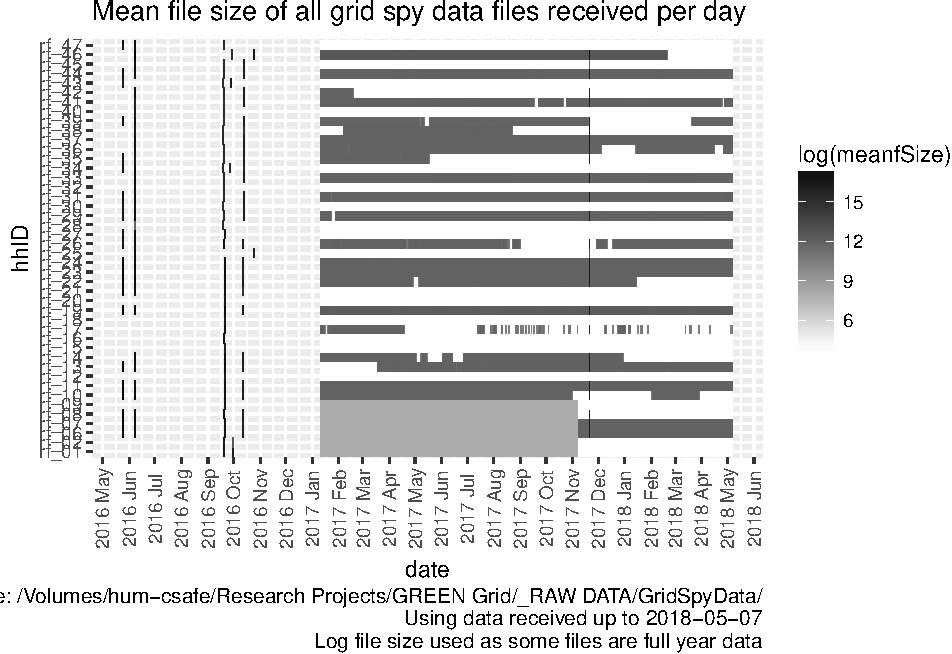
\includegraphics{processNZGGElecCons1minData_files/figure-latex/allFileSizesPlot-1.pdf}

\begin{Shaded}
\begin{Highlighting}[]
\KeywordTok{ggsave}\NormalTok{(}\KeywordTok{paste0}\NormalTok{(outPath, }\StringTok{"gridSpyAllFileListSizeTilePlot.png"}\NormalTok{))}
\end{Highlighting}
\end{Shaded}

\begin{verbatim}
## Saving 6.5 x 4.5 in image
\end{verbatim}

The following chart shows the same chart but only for files which we
think contain data.

\begin{Shaded}
\begin{Highlighting}[]
\NormalTok{myCaption <-}\StringTok{ }\KeywordTok{paste0}\NormalTok{(}\StringTok{"Data source: "}\NormalTok{, fpath,}
                    \StringTok{"}\CharTok{\textbackslash{}n}\StringTok{Using data received up to "}\NormalTok{, }\KeywordTok{Sys.Date}\NormalTok{())}

\NormalTok{plotDT <-}\StringTok{ }\NormalTok{fListCompleteDT[}\OperatorTok{!}\KeywordTok{is.na}\NormalTok{(dateFormat), .(}\DataTypeTok{nFiles =}\NormalTok{ .N,}
                              \DataTypeTok{meanfSize =} \KeywordTok{mean}\NormalTok{(fSize)), }
\NormalTok{                          keyby =}\StringTok{ }\NormalTok{.(hhID, }\DataTypeTok{date =} \KeywordTok{as.Date}\NormalTok{(fMDate))]}

\KeywordTok{ggplot}\NormalTok{(plotDT, }\KeywordTok{aes}\NormalTok{( }\DataTypeTok{x =}\NormalTok{ date, }\DataTypeTok{y =}\NormalTok{ hhID, }\DataTypeTok{fill =} \KeywordTok{log}\NormalTok{(meanfSize))) }\OperatorTok{+}
\StringTok{  }\KeywordTok{geom_tile}\NormalTok{() }\OperatorTok{+}
\StringTok{  }\KeywordTok{scale_fill_gradient}\NormalTok{(}\DataTypeTok{low =} \StringTok{"white"}\NormalTok{, }\DataTypeTok{high =} \StringTok{"black"}\NormalTok{) }\OperatorTok{+}\StringTok{ }
\StringTok{  }\KeywordTok{scale_x_date}\NormalTok{(}\DataTypeTok{date_labels =} \StringTok{"%Y %b"}\NormalTok{, }\DataTypeTok{date_breaks =} \StringTok{"1 month"}\NormalTok{) }\OperatorTok{+}
\StringTok{  }\KeywordTok{theme}\NormalTok{(}\DataTypeTok{axis.text.x =} \KeywordTok{element_text}\NormalTok{(}\DataTypeTok{angle =} \DecValTok{90}\NormalTok{, }\DataTypeTok{vjust =} \FloatTok{0.5}\NormalTok{, }\DataTypeTok{hjust =} \FloatTok{0.5}\NormalTok{)) }\OperatorTok{+}\StringTok{ }
\StringTok{  }\KeywordTok{labs}\NormalTok{(}\DataTypeTok{title =} \StringTok{"Mean file size of loaded grid spy data files received per day"}\NormalTok{,}
       \DataTypeTok{caption =} \KeywordTok{paste0}\NormalTok{(myCaption, }
                        \StringTok{"}\CharTok{\textbackslash{}n}\StringTok{Log file size used as some files are full year data"}\NormalTok{,}
                        \StringTok{"}\CharTok{\textbackslash{}n}\StringTok{Files loaded if fsize > "}\NormalTok{, dataThreshold, }\StringTok{" bytes"}\NormalTok{)}
    
\NormalTok{  )}
\end{Highlighting}
\end{Shaded}

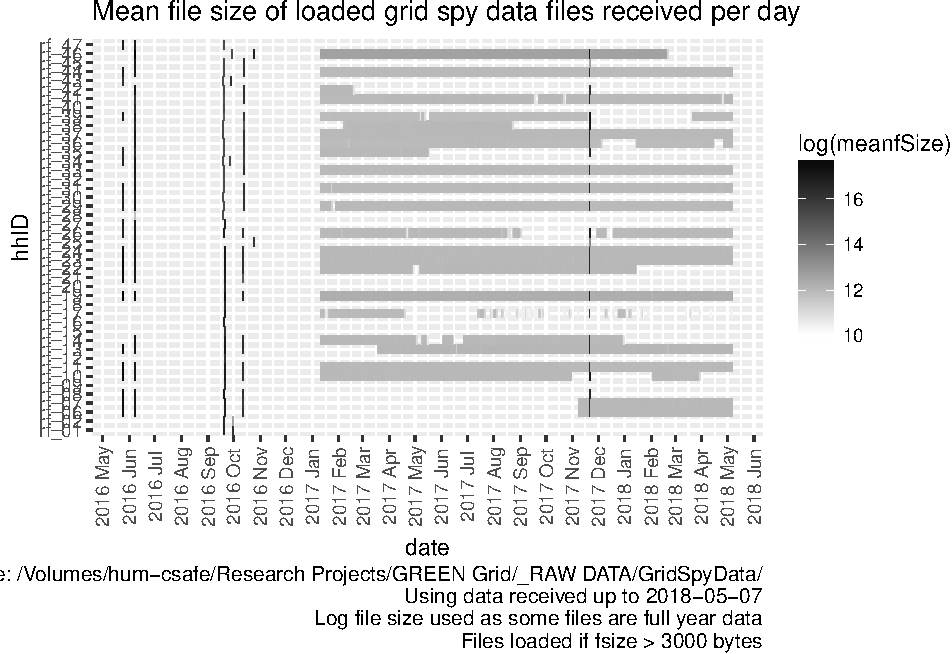
\includegraphics{processNZGGElecCons1minData_files/figure-latex/loadedFileSizesPlot-1.pdf}

\begin{Shaded}
\begin{Highlighting}[]
\KeywordTok{ggsave}\NormalTok{(}\KeywordTok{paste0}\NormalTok{(outPath, }\StringTok{"gridSpyLoadedFileListSizeTilePlot.png"}\NormalTok{))}
\end{Highlighting}
\end{Shaded}

\begin{verbatim}
## Saving 6.5 x 4.5 in image
\end{verbatim}

\section{Load data files}\label{load-data-files}

In this section we load the data files that have a file size
\textgreater{} 3000 bytes. Things to note:

\begin{itemize}
\tightlist
\item
  We assume that any files smaller than this value have no observations.
  This is based on:

  \begin{itemize}
  \tightlist
  \item
    Manual inspection of several small files
  \item
    The identical (small) file sizes involved
  \item
    \emph{But} we should probably test the first few lines to double
    check\ldots{}
  \end{itemize}
\item
  We have to deal with quite a lot of duplication some of which has
  caused the different date formats. See our
  \href{https://git.soton.ac.uk/ba1e12/nzGREENGrid/issues?scope=all\&utf8=\%E2\%9C\%93\&state=all}{repo
  issues list}.
\end{itemize}

The following table shows the number of files per household that we
willl load.

\begin{Shaded}
\begin{Highlighting}[]
\NormalTok{filesToLoadDT <-}\StringTok{ }\NormalTok{fListCompleteDT[}\OperatorTok{!}\KeywordTok{is.na}\NormalTok{(dateFormat)]}

\NormalTok{t <-}\StringTok{ }\NormalTok{filesToLoadDT[, .(}\DataTypeTok{nFiles =}\NormalTok{ .N,}
                       \DataTypeTok{meanSize =} \KeywordTok{mean}\NormalTok{(fSize),}
                       \DataTypeTok{minFileDate =} \KeywordTok{min}\NormalTok{(fMDate),}
                       \DataTypeTok{maxFileDate =} \KeywordTok{max}\NormalTok{(fMDate)), keyby =}\StringTok{ }\NormalTok{.(hhID)]}

\KeywordTok{kable}\NormalTok{(}\DataTypeTok{caption =} \StringTok{"Summary of household files to load"}\NormalTok{, t)}
\end{Highlighting}
\end{Shaded}

\begin{longtable}[]{@{}lrrll@{}}
\caption{Summary of household files to load}\tabularnewline
\toprule
hhID & nFiles & meanSize & minFileDate & maxFileDate\tabularnewline
\midrule
\endfirsthead
\toprule
hhID & nFiles & meanSize & minFileDate & maxFileDate\tabularnewline
\midrule
\endhead
rf\_01 & 3 & 15548174.7 & 2016-09-20 & 2016-09-30\tabularnewline
rf\_02 & 3 & 10134268.3 & 2016-09-20 & 2016-09-30\tabularnewline
rf\_06 & 184 & 796993.1 & 2016-05-25 & 2018-05-06\tabularnewline
rf\_07 & 184 & 856408.8 & 2016-05-25 & 2018-05-06\tabularnewline
rf\_08 & 5 & 23989121.0 & 2016-05-25 & 2017-11-21\tabularnewline
rf\_09 & 2 & 14344605.0 & 2016-09-21 & 2016-09-21\tabularnewline
rf\_10 & 358 & 525455.0 & 2016-05-25 & 2018-03-30\tabularnewline
rf\_11 & 486 & 425513.4 & 2016-05-25 & 2018-05-06\tabularnewline
rf\_12 & 2 & 10713096.0 & 2016-09-21 & 2016-09-21\tabularnewline
rf\_13 & 418 & 492196.3 & 2016-05-25 & 2018-05-06\tabularnewline
rf\_14 & 329 & 424262.0 & 2016-06-08 & 2017-12-31\tabularnewline
rf\_15 & 2 & 10553143.0 & 2016-09-21 & 2016-09-21\tabularnewline
rf\_16 & 1 & 20037376.0 & 2016-09-20 & 2016-09-20\tabularnewline
rf\_17 & 204 & 411367.1 & 2016-09-21 & 2018-05-06\tabularnewline
rf\_18 & 2 & 14374309.5 & 2016-09-21 & 2016-09-21\tabularnewline
rf\_19 & 486 & 564919.2 & 2016-05-25 & 2018-05-06\tabularnewline
rf\_20 & 2 & 14665810.0 & 2016-09-21 & 2016-09-21\tabularnewline
rf\_21 & 4 & 23058797.8 & 2016-05-25 & 2016-10-12\tabularnewline
rf\_22 & 371 & 533704.5 & 2016-05-25 & 2018-01-16\tabularnewline
rf\_23 & 486 & 441146.7 & 2016-05-25 & 2018-05-06\tabularnewline
rf\_24 & 486 & 429596.2 & 2016-05-25 & 2018-05-06\tabularnewline
rf\_25 & 3 & 12341581.3 & 2016-06-08 & 2017-11-21\tabularnewline
rf\_26 & 392 & 409680.3 & 2016-05-25 & 2018-05-06\tabularnewline
rf\_27 & 3 & 22607698.7 & 2016-05-25 & 2016-09-21\tabularnewline
rf\_28 & 2 & 2297483.0 & 2016-06-08 & 2016-09-19\tabularnewline
rf\_29 & 483 & 341817.2 & 2016-05-25 & 2018-05-06\tabularnewline
rf\_30 & 5 & 13695336.0 & 2016-05-25 & 2016-10-13\tabularnewline
rf\_31 & 486 & 341010.9 & 2016-05-25 & 2018-05-06\tabularnewline
rf\_32 & 2 & 13934454.0 & 2016-06-08 & 2016-09-20\tabularnewline
rf\_33 & 485 & 287829.0 & 2016-06-08 & 2018-05-06\tabularnewline
rf\_34 & 7 & 14106275.3 & 2016-05-25 & 2016-10-13\tabularnewline
rf\_35 & 134 & 573648.6 & 2016-05-25 & 2017-11-21\tabularnewline
rf\_36 & 436 & 300565.6 & 2016-06-08 & 2018-05-06\tabularnewline
rf\_37 & 485 & 301672.8 & 2016-06-08 & 2018-05-06\tabularnewline
rf\_38 & 201 & 385707.5 & 2016-06-08 & 2017-11-21\tabularnewline
rf\_39 & 362 & 382595.6 & 2016-05-25 & 2018-05-06\tabularnewline
rf\_40 & 2 & 9299902.0 & 2016-06-08 & 2016-09-20\tabularnewline
rf\_41 & 477 & 265329.0 & 2016-06-08 & 2018-05-06\tabularnewline
rf\_42 & 45 & 1315953.6 & 2016-06-08 & 2017-11-21\tabularnewline
rf\_43 & 4 & 9442492.0 & 2016-05-25 & 2016-09-28\tabularnewline
rf\_44 & 486 & 342616.0 & 2016-05-25 & 2018-05-06\tabularnewline
rf\_45 & 4 & 10513812.0 & 2016-06-08 & 2017-11-21\tabularnewline
rf\_46 & 411 & 605048.1 & 2016-06-08 & 2018-02-21\tabularnewline
rf\_47 & 3 & 17544847.0 & 2016-05-25 & 2016-09-20\tabularnewline
\bottomrule
\end{longtable}

\begin{Shaded}
\begin{Highlighting}[]
\CommentTok{# > Load, process & save the ones which probably have data ----}
\NormalTok{fListCompleteDT <-}\StringTok{ }\NormalTok{fListCompleteDT[, fileLoaded }\OperatorTok{:}\ErrorTok{=}\StringTok{ "No"}\NormalTok{] }\CommentTok{# set default}
\NormalTok{hhIDs <-}\StringTok{ }\KeywordTok{unique}\NormalTok{(filesToLoadDT}\OperatorTok{$}\NormalTok{hhID) }\CommentTok{# list of household ids}
\NormalTok{hhStatDT <-}\StringTok{ }\KeywordTok{data.table}\NormalTok{() }\CommentTok{# stats collector}

\ControlFlowTok{for}\NormalTok{(hh }\ControlFlowTok{in}\NormalTok{ hhIDs)\{}
\NormalTok{  tempHhDT <-}\StringTok{ }\KeywordTok{data.table}\NormalTok{() }\CommentTok{# hh data collector}
  \KeywordTok{print}\NormalTok{(}\KeywordTok{paste0}\NormalTok{(}\StringTok{"Loading: "}\NormalTok{, hh))}
\NormalTok{  filesToLoad <-}\StringTok{ }\NormalTok{filesToLoadDT[hhID }\OperatorTok{==}\StringTok{ }\NormalTok{hh, fullPath]}
  \ControlFlowTok{for}\NormalTok{(f }\ControlFlowTok{in}\NormalTok{ filesToLoad)\{}
    \ControlFlowTok{if}\NormalTok{(fullFb)\{}\KeywordTok{print}\NormalTok{(}\KeywordTok{paste0}\NormalTok{(}\StringTok{"File size ("}\NormalTok{, f, }\StringTok{") = "}\NormalTok{, }
\NormalTok{                            filesToLoadDT[fullPath }\OperatorTok{==}\StringTok{ }\NormalTok{f, fSize], }
                            \StringTok{" so probably OK"}\NormalTok{))\} }\CommentTok{# files under 3kb are probably empty}
    \CommentTok{# attempt to load the file}
\NormalTok{    tempDT <-}\StringTok{ }\KeywordTok{fread}\NormalTok{(f)}
    \ControlFlowTok{if}\NormalTok{(fullFb)\{}\KeywordTok{print}\NormalTok{(}\StringTok{"File loaded"}\NormalTok{)\}}
    \CommentTok{# set some file stats}
\NormalTok{    fListCompleteDT <-}\StringTok{ }\NormalTok{fListCompleteDT[fullPath }\OperatorTok{==}\StringTok{ }\NormalTok{f, fileLoaded }\OperatorTok{:}\ErrorTok{=}\StringTok{ "Yes"}\NormalTok{]}
\NormalTok{    fListCompleteDT <-}\StringTok{ }\NormalTok{fListCompleteDT[fullPath }\OperatorTok{==}\StringTok{ }\NormalTok{f, nObs }\OperatorTok{:}\ErrorTok{=}\StringTok{ }\KeywordTok{nrow}\NormalTok{(tempDT)] }\CommentTok{# could include duplicates}
    
    \CommentTok{# what is the date column called?}
      \ControlFlowTok{if}\NormalTok{(}\KeywordTok{nrow}\NormalTok{(}\KeywordTok{select}\NormalTok{(tempDT, }\KeywordTok{contains}\NormalTok{(}\StringTok{"NZ"}\NormalTok{))) }\OperatorTok{>}\StringTok{ }\DecValTok{0}\NormalTok{)\{ }\CommentTok{# requires dplyr}
        \KeywordTok{setnames}\NormalTok{(tempDT, }\StringTok{'date NZ'}\NormalTok{, }\StringTok{"dateTime_char"}\NormalTok{)}
\NormalTok{        tempDT <-}\StringTok{ }\NormalTok{tempDT[, dateColName }\OperatorTok{:}\ErrorTok{=}\StringTok{ "date NZ"}\NormalTok{]}
\NormalTok{      \} }
      \ControlFlowTok{if}\NormalTok{(}\KeywordTok{nrow}\NormalTok{(}\KeywordTok{select}\NormalTok{(tempDT, }\KeywordTok{contains}\NormalTok{(}\StringTok{"UTC"}\NormalTok{))) }\OperatorTok{>}\StringTok{ }\DecValTok{0}\NormalTok{)\{ }\CommentTok{# requires dplyr}
        \KeywordTok{setnames}\NormalTok{(tempDT, }\StringTok{'date UTC'}\NormalTok{, }\StringTok{"dateTime_char"}\NormalTok{)}
\NormalTok{        tempDT <-}\StringTok{ }\NormalTok{tempDT[, dateColName }\OperatorTok{:}\ErrorTok{=}\StringTok{ "date UTC"}\NormalTok{]}
\NormalTok{      \}}
      
      \CommentTok{# Now use the pre-inferred dateFormat}
\NormalTok{      tempDT <-}\StringTok{ }\NormalTok{tempDT[, dateFormat }\OperatorTok{:}\ErrorTok{=}\StringTok{ }\NormalTok{filesToLoadDT[fullPath }\OperatorTok{==}\StringTok{ }\NormalTok{f, dateFormat]]}
\NormalTok{      tempDT <-}\StringTok{ }\NormalTok{tempDT[dateFormat }\OperatorTok\StringTok{ "mdy"} \OperatorTok{&}\StringTok{ }\NormalTok{dateColName }\OperatorTok\StringTok{ "NZ"}\NormalTok{, r_dateTime }\OperatorTok{:}\ErrorTok{=}\StringTok{ }\KeywordTok{mdy_hm}\NormalTok{(dateTime_char, }\DataTypeTok{tz =} \StringTok{"Pacific/Auckland"}\NormalTok{)] }\CommentTok{# requires lubridate}
\NormalTok{      tempDT <-}\StringTok{ }\NormalTok{tempDT[dateFormat }\OperatorTok\StringTok{ "dmy"} \OperatorTok{&}\StringTok{ }\NormalTok{dateColName }\OperatorTok\StringTok{ "NZ"}\NormalTok{, r_dateTime }\OperatorTok{:}\ErrorTok{=}\StringTok{ }\KeywordTok{dmy_hm}\NormalTok{(dateTime_char, }\DataTypeTok{tz =} \StringTok{"Pacific/Auckland"}\NormalTok{)] }\CommentTok{# requires lubridate}
\NormalTok{      tempDT <-}\StringTok{ }\NormalTok{tempDT[dateFormat }\OperatorTok\StringTok{ "ydm"} \OperatorTok{&}\StringTok{ }\NormalTok{dateColName }\OperatorTok\StringTok{ "NZ"}\NormalTok{, r_dateTime }\OperatorTok{:}\ErrorTok{=}\StringTok{ }\KeywordTok{ymd_hm}\NormalTok{(dateTime_char, }\DataTypeTok{tz =} \StringTok{"Pacific/Auckland"}\NormalTok{)] }\CommentTok{# requires lubridate}
\NormalTok{      tempDT <-}\StringTok{ }\NormalTok{tempDT[dateFormat }\OperatorTok\StringTok{ "ymd"} \OperatorTok{&}\StringTok{ }\NormalTok{dateColName }\OperatorTok\StringTok{ "NZ"}\NormalTok{, r_dateTime }\OperatorTok{:}\ErrorTok{=}\StringTok{ }\KeywordTok{ymd_hm}\NormalTok{(dateTime_char, }\DataTypeTok{tz =} \StringTok{"Pacific/Auckland"}\NormalTok{)] }\CommentTok{# requires lubridate}
\NormalTok{      tempDT <-}\StringTok{ }\NormalTok{tempDT[dateFormat }\OperatorTok\StringTok{ "mdy"} \OperatorTok{&}\StringTok{ }\NormalTok{dateColName }\OperatorTok\StringTok{ "UTC"}\NormalTok{, r_dateTime }\OperatorTok{:}\ErrorTok{=}\StringTok{ }\KeywordTok{mdy_hm}\NormalTok{(dateTime_char, }\DataTypeTok{tz =} \StringTok{"UTC"}\NormalTok{)] }\CommentTok{# requires lubridate}
\NormalTok{      tempDT <-}\StringTok{ }\NormalTok{tempDT[dateFormat }\OperatorTok\StringTok{ "dmy"} \OperatorTok{&}\StringTok{ }\NormalTok{dateColName }\OperatorTok\StringTok{ "UTC"}\NormalTok{, r_dateTime }\OperatorTok{:}\ErrorTok{=}\StringTok{ }\KeywordTok{dmy_hm}\NormalTok{(dateTime_char, }\DataTypeTok{tz =} \StringTok{"UTC"}\NormalTok{)] }\CommentTok{# requires lubridate}
\NormalTok{      tempDT <-}\StringTok{ }\NormalTok{tempDT[dateFormat }\OperatorTok\StringTok{ "ydm"} \OperatorTok{&}\StringTok{ }\NormalTok{dateColName }\OperatorTok\StringTok{ "UTC"}\NormalTok{, r_dateTime }\OperatorTok{:}\ErrorTok{=}\StringTok{ }\KeywordTok{ymd_hm}\NormalTok{(dateTime_char, }\DataTypeTok{tz =} \StringTok{"UTC"}\NormalTok{)] }\CommentTok{# requires lubridate}
\NormalTok{      tempDT <-}\StringTok{ }\NormalTok{tempDT[dateFormat }\OperatorTok\StringTok{ "ymd"} \OperatorTok{&}\StringTok{ }\NormalTok{dateColName }\OperatorTok\StringTok{ "UTC"}\NormalTok{, r_dateTime }\OperatorTok{:}\ErrorTok{=}\StringTok{ }\KeywordTok{ymd_hm}\NormalTok{(dateTime_char, }\DataTypeTok{tz =} \StringTok{"UTC"}\NormalTok{)] }\CommentTok{# requires lubridate}
      \ControlFlowTok{if}\NormalTok{(fullFb)\{}
        \KeywordTok{print}\NormalTok{(}\KeywordTok{head}\NormalTok{(tempDT))}
        \KeywordTok{print}\NormalTok{(}\KeywordTok{summary}\NormalTok{(tempDT))}
        \CommentTok{#print(table(tempDT$dateFormat))}
\NormalTok{        \}}
    
\NormalTok{    fListCompleteDT <-}\StringTok{ }\NormalTok{fListCompleteDT[fullPath }\OperatorTok{==}\StringTok{ }\NormalTok{f, obsStartDate }\OperatorTok{:}\ErrorTok{=}\StringTok{ }\KeywordTok{min}\NormalTok{(}\KeywordTok{as.Date}\NormalTok{(tempDT}\OperatorTok{$}\NormalTok{r_dateTime))] }\CommentTok{# should be a sensible number and not NA}
\NormalTok{    fListCompleteDT <-}\StringTok{ }\NormalTok{fListCompleteDT[fullPath }\OperatorTok{==}\StringTok{ }\NormalTok{f, obsEndDate }\OperatorTok{:}\ErrorTok{=}\StringTok{ }\KeywordTok{max}\NormalTok{(}\KeywordTok{as.Date}\NormalTok{(tempDT}\OperatorTok{$}\NormalTok{r_dateTime))] }\CommentTok{# should be a sensible number and not NA}
\NormalTok{    fListCompleteDT <-}\StringTok{ }\NormalTok{fListCompleteDT[fullPath }\OperatorTok{==}\StringTok{ }\NormalTok{f, nCircuits }\OperatorTok{:}\ErrorTok{=}\StringTok{ }\KeywordTok{ncol}\NormalTok{(}\KeywordTok{select}\NormalTok{(tempDT, }\KeywordTok{contains}\NormalTok{(}\StringTok{"$"}\NormalTok{)))] }\CommentTok{# check for the number of circuits - all seem to contain "$"}
\NormalTok{    tempHhDT <-}\StringTok{ }\KeywordTok{rbind}\NormalTok{(tempHhDT, tempDT, }\DataTypeTok{fill =} \OtherTok{TRUE}\NormalTok{) }\CommentTok{# just in case there are different numbers of columns (quite likely!)}
\NormalTok{  \}}
  
  \CommentTok{# > Remove duplicates caused by over-lapping files and dates etc ----}
  \CommentTok{# Need to remove all uneccessary vars for this}
  \KeywordTok{try}\NormalTok{(tempHhDT}\OperatorTok{$}\NormalTok{dateColName <-}\StringTok{ }\OtherTok{NULL}\NormalTok{)}
  \KeywordTok{try}\NormalTok{(tempHhDT}\OperatorTok{$}\NormalTok{dateFormat <-}\StringTok{ }\OtherTok{NULL}\NormalTok{)}
  \KeywordTok{try}\NormalTok{(tempHhDT}\OperatorTok{$}\NormalTok{nCircuits <-}\StringTok{ }\OtherTok{NULL}\NormalTok{)}
  \KeywordTok{try}\NormalTok{(tempHhDT}\OperatorTok{$}\NormalTok{dateTime_char <-}\StringTok{ }\OtherTok{NULL}\NormalTok{) }\CommentTok{# if we leave this one in then we get duplciates where we have date NZ & date UTC for the same timestamp due to overlapping file downloads}
  
\NormalTok{  nObs <-}\StringTok{ }\KeywordTok{nrow}\NormalTok{(tempHhDT)}
  \ControlFlowTok{if}\NormalTok{(fullFb)\{}\KeywordTok{print}\NormalTok{(}\KeywordTok{paste0}\NormalTok{(}\StringTok{"N rows before removal of duplicates: "}\NormalTok{, nObs))\}}
\NormalTok{  tempHhDT <-}\StringTok{ }\KeywordTok{unique}\NormalTok{(tempHhDT)}
\NormalTok{  nObs <-}\StringTok{ }\KeywordTok{nrow}\NormalTok{(tempHhDT)}
  \ControlFlowTok{if}\NormalTok{(fullFb)\{}\KeywordTok{print}\NormalTok{(}\KeywordTok{paste0}\NormalTok{(}\StringTok{"N rows after removal of duplicates: "}\NormalTok{, nObs))\}}
  
\NormalTok{  hhStatTempDT <-}\StringTok{ }\NormalTok{tempHhDT[, .(}\DataTypeTok{nObs =}\NormalTok{ .N,}
                           \DataTypeTok{nDataColumns =} \KeywordTok{ncol}\NormalTok{(}\KeywordTok{select}\NormalTok{(tempDT, }\KeywordTok{contains}\NormalTok{(}\StringTok{"$"}\NormalTok{)))), }\CommentTok{# the actual number of columns in the whole household file with "$" in them in case of rbind "errors" caused by files with different column names}
\NormalTok{                           keyby =}\StringTok{ }\NormalTok{(}\DataTypeTok{date =} \KeywordTok{as.Date}\NormalTok{(r_dateTime))] }\CommentTok{# can't do sensible summary stats on W as some circuits are sub-sets of others!}
  \CommentTok{# add hhID}
\NormalTok{  hhStatTempDT <-}\StringTok{ }\NormalTok{hhStatTempDT[, hhID }\OperatorTok{:}\ErrorTok{=}\StringTok{ }\NormalTok{hh]}
  
\NormalTok{  hhStatDT <-}\StringTok{ }\KeywordTok{rbind}\NormalTok{(hhStatDT,hhStatTempDT) }\CommentTok{# add to the collector}
  
  \CommentTok{# > Save hh file ----}
  
\NormalTok{  ofile <-}\StringTok{ }\KeywordTok{paste0}\NormalTok{(outPath, }\StringTok{"data/"}\NormalTok{, hh,}\StringTok{"_all_1min_data.csv"}\NormalTok{)}
  \KeywordTok{print}\NormalTok{(}\KeywordTok{paste0}\NormalTok{(}\StringTok{"Saving "}\NormalTok{, ofile, }\StringTok{"..."}\NormalTok{))}
  \KeywordTok{write_csv}\NormalTok{(tempHhDT, ofile)}
  \KeywordTok{print}\NormalTok{(}\KeywordTok{paste0}\NormalTok{(}\StringTok{"Saved "}\NormalTok{, ofile, }\StringTok{", gzipping..."}\NormalTok{))}
  
\NormalTok{  cmd <-}\StringTok{ }\KeywordTok{paste0}\NormalTok{(}\StringTok{"gzip -f "}\NormalTok{, }\StringTok{"'"}\NormalTok{, }\KeywordTok{path.expand}\NormalTok{(ofile), }\StringTok{"'"}\NormalTok{) }\CommentTok{# gzip it - use quotes in case of spaces in file name, expand path if needed}
  \KeywordTok{try}\NormalTok{(}\KeywordTok{system}\NormalTok{(cmd)) }\CommentTok{# in case it fails - if it does there will just be .csv files (not gzipped) - e.g. under windows}
  \KeywordTok{print}\NormalTok{(}\KeywordTok{paste0}\NormalTok{(}\StringTok{"Gzipped "}\NormalTok{, ofile))}
  
    \ControlFlowTok{if}\NormalTok{(fullFb)\{}
    \KeywordTok{print}\NormalTok{(}\StringTok{"Col names: "}\NormalTok{)}
    \KeywordTok{print}\NormalTok{(}\KeywordTok{names}\NormalTok{(tempHhDT))}
\NormalTok{    \}}
  
\NormalTok{  tempHhDT <-}\StringTok{ }\OtherTok{NULL} \CommentTok{# just in case}
\NormalTok{\}}
\end{Highlighting}
\end{Shaded}

\begin{verbatim}
## [1] "Loading: rf_01"
\end{verbatim}

\begin{verbatim}
## Warning in `[<-.data.table`(x, j = name, value = value): Adding new column
## 'nCircuits' then assigning NULL (deleting it).
\end{verbatim}

\begin{verbatim}
## [1] "Saving /Volumes/hum-csafe/Research Projects/GREEN Grid/Clean_data/gridSpy/1min/data/rf_01_all_1min_data.csv..."
## [1] "Saved /Volumes/hum-csafe/Research Projects/GREEN Grid/Clean_data/gridSpy/1min/data/rf_01_all_1min_data.csv, gzipping..."
## [1] "Gzipped /Volumes/hum-csafe/Research Projects/GREEN Grid/Clean_data/gridSpy/1min/data/rf_01_all_1min_data.csv"
## [1] "Loading: rf_02"
\end{verbatim}

\begin{verbatim}
## Warning in `[<-.data.table`(x, j = name, value = value): Adding new column
## 'nCircuits' then assigning NULL (deleting it).
\end{verbatim}

\begin{verbatim}
## [1] "Saving /Volumes/hum-csafe/Research Projects/GREEN Grid/Clean_data/gridSpy/1min/data/rf_02_all_1min_data.csv..."
## [1] "Saved /Volumes/hum-csafe/Research Projects/GREEN Grid/Clean_data/gridSpy/1min/data/rf_02_all_1min_data.csv, gzipping..."
## [1] "Gzipped /Volumes/hum-csafe/Research Projects/GREEN Grid/Clean_data/gridSpy/1min/data/rf_02_all_1min_data.csv"
## [1] "Loading: rf_06"
\end{verbatim}

\begin{verbatim}
## Warning in `[<-.data.table`(x, j = name, value = value): Adding new column
## 'nCircuits' then assigning NULL (deleting it).
\end{verbatim}

\begin{verbatim}
## [1] "Saving /Volumes/hum-csafe/Research Projects/GREEN Grid/Clean_data/gridSpy/1min/data/rf_06_all_1min_data.csv..."
## [1] "Saved /Volumes/hum-csafe/Research Projects/GREEN Grid/Clean_data/gridSpy/1min/data/rf_06_all_1min_data.csv, gzipping..."
## [1] "Gzipped /Volumes/hum-csafe/Research Projects/GREEN Grid/Clean_data/gridSpy/1min/data/rf_06_all_1min_data.csv"
## [1] "Loading: rf_07"
\end{verbatim}

\begin{verbatim}
## Warning in `[<-.data.table`(x, j = name, value = value): Adding new column
## 'nCircuits' then assigning NULL (deleting it).
\end{verbatim}

\begin{verbatim}
## [1] "Saving /Volumes/hum-csafe/Research Projects/GREEN Grid/Clean_data/gridSpy/1min/data/rf_07_all_1min_data.csv..."
## [1] "Saved /Volumes/hum-csafe/Research Projects/GREEN Grid/Clean_data/gridSpy/1min/data/rf_07_all_1min_data.csv, gzipping..."
## [1] "Gzipped /Volumes/hum-csafe/Research Projects/GREEN Grid/Clean_data/gridSpy/1min/data/rf_07_all_1min_data.csv"
## [1] "Loading: rf_08"
\end{verbatim}

\begin{verbatim}
## Warning in `[<-.data.table`(x, j = name, value = value): Adding new column
## 'nCircuits' then assigning NULL (deleting it).
\end{verbatim}

\begin{verbatim}
## [1] "Saving /Volumes/hum-csafe/Research Projects/GREEN Grid/Clean_data/gridSpy/1min/data/rf_08_all_1min_data.csv..."
## [1] "Saved /Volumes/hum-csafe/Research Projects/GREEN Grid/Clean_data/gridSpy/1min/data/rf_08_all_1min_data.csv, gzipping..."
## [1] "Gzipped /Volumes/hum-csafe/Research Projects/GREEN Grid/Clean_data/gridSpy/1min/data/rf_08_all_1min_data.csv"
## [1] "Loading: rf_09"
\end{verbatim}

\begin{verbatim}
## Warning in `[<-.data.table`(x, j = name, value = value): Adding new column
## 'nCircuits' then assigning NULL (deleting it).
\end{verbatim}

\begin{verbatim}
## [1] "Saving /Volumes/hum-csafe/Research Projects/GREEN Grid/Clean_data/gridSpy/1min/data/rf_09_all_1min_data.csv..."
## [1] "Saved /Volumes/hum-csafe/Research Projects/GREEN Grid/Clean_data/gridSpy/1min/data/rf_09_all_1min_data.csv, gzipping..."
## [1] "Gzipped /Volumes/hum-csafe/Research Projects/GREEN Grid/Clean_data/gridSpy/1min/data/rf_09_all_1min_data.csv"
## [1] "Loading: rf_10"
\end{verbatim}

\begin{verbatim}
## Warning in `[<-.data.table`(x, j = name, value = value): Adding new column
## 'nCircuits' then assigning NULL (deleting it).
\end{verbatim}

\begin{verbatim}
## [1] "Saving /Volumes/hum-csafe/Research Projects/GREEN Grid/Clean_data/gridSpy/1min/data/rf_10_all_1min_data.csv..."
## [1] "Saved /Volumes/hum-csafe/Research Projects/GREEN Grid/Clean_data/gridSpy/1min/data/rf_10_all_1min_data.csv, gzipping..."
## [1] "Gzipped /Volumes/hum-csafe/Research Projects/GREEN Grid/Clean_data/gridSpy/1min/data/rf_10_all_1min_data.csv"
## [1] "Loading: rf_11"
\end{verbatim}

\begin{verbatim}
## Warning in `[<-.data.table`(x, j = name, value = value): Adding new column
## 'nCircuits' then assigning NULL (deleting it).
\end{verbatim}

\begin{verbatim}
## [1] "Saving /Volumes/hum-csafe/Research Projects/GREEN Grid/Clean_data/gridSpy/1min/data/rf_11_all_1min_data.csv..."
## [1] "Saved /Volumes/hum-csafe/Research Projects/GREEN Grid/Clean_data/gridSpy/1min/data/rf_11_all_1min_data.csv, gzipping..."
## [1] "Gzipped /Volumes/hum-csafe/Research Projects/GREEN Grid/Clean_data/gridSpy/1min/data/rf_11_all_1min_data.csv"
## [1] "Loading: rf_12"
\end{verbatim}

\begin{verbatim}
## Warning in `[<-.data.table`(x, j = name, value = value): Adding new column
## 'nCircuits' then assigning NULL (deleting it).
\end{verbatim}

\begin{verbatim}
## [1] "Saving /Volumes/hum-csafe/Research Projects/GREEN Grid/Clean_data/gridSpy/1min/data/rf_12_all_1min_data.csv..."
## [1] "Saved /Volumes/hum-csafe/Research Projects/GREEN Grid/Clean_data/gridSpy/1min/data/rf_12_all_1min_data.csv, gzipping..."
## [1] "Gzipped /Volumes/hum-csafe/Research Projects/GREEN Grid/Clean_data/gridSpy/1min/data/rf_12_all_1min_data.csv"
## [1] "Loading: rf_13"
\end{verbatim}

\begin{verbatim}
## Warning in `[<-.data.table`(x, j = name, value = value): Adding new column
## 'nCircuits' then assigning NULL (deleting it).
\end{verbatim}

\begin{verbatim}
## [1] "Saving /Volumes/hum-csafe/Research Projects/GREEN Grid/Clean_data/gridSpy/1min/data/rf_13_all_1min_data.csv..."
## [1] "Saved /Volumes/hum-csafe/Research Projects/GREEN Grid/Clean_data/gridSpy/1min/data/rf_13_all_1min_data.csv, gzipping..."
## [1] "Gzipped /Volumes/hum-csafe/Research Projects/GREEN Grid/Clean_data/gridSpy/1min/data/rf_13_all_1min_data.csv"
## [1] "Loading: rf_14"
\end{verbatim}

\begin{verbatim}
## Warning in `[<-.data.table`(x, j = name, value = value): Adding new column
## 'nCircuits' then assigning NULL (deleting it).
\end{verbatim}

\begin{verbatim}
## [1] "Saving /Volumes/hum-csafe/Research Projects/GREEN Grid/Clean_data/gridSpy/1min/data/rf_14_all_1min_data.csv..."
## [1] "Saved /Volumes/hum-csafe/Research Projects/GREEN Grid/Clean_data/gridSpy/1min/data/rf_14_all_1min_data.csv, gzipping..."
## [1] "Gzipped /Volumes/hum-csafe/Research Projects/GREEN Grid/Clean_data/gridSpy/1min/data/rf_14_all_1min_data.csv"
## [1] "Loading: rf_15"
\end{verbatim}

\begin{verbatim}
## Warning in `[<-.data.table`(x, j = name, value = value): Adding new column
## 'nCircuits' then assigning NULL (deleting it).
\end{verbatim}

\begin{verbatim}
## [1] "Saving /Volumes/hum-csafe/Research Projects/GREEN Grid/Clean_data/gridSpy/1min/data/rf_15_all_1min_data.csv..."
## [1] "Saved /Volumes/hum-csafe/Research Projects/GREEN Grid/Clean_data/gridSpy/1min/data/rf_15_all_1min_data.csv, gzipping..."
## [1] "Gzipped /Volumes/hum-csafe/Research Projects/GREEN Grid/Clean_data/gridSpy/1min/data/rf_15_all_1min_data.csv"
## [1] "Loading: rf_16"
\end{verbatim}

\begin{verbatim}
## Warning in `[<-.data.table`(x, j = name, value = value): Adding new column
## 'nCircuits' then assigning NULL (deleting it).
\end{verbatim}

\begin{verbatim}
## [1] "Saving /Volumes/hum-csafe/Research Projects/GREEN Grid/Clean_data/gridSpy/1min/data/rf_16_all_1min_data.csv..."
## [1] "Saved /Volumes/hum-csafe/Research Projects/GREEN Grid/Clean_data/gridSpy/1min/data/rf_16_all_1min_data.csv, gzipping..."
## [1] "Gzipped /Volumes/hum-csafe/Research Projects/GREEN Grid/Clean_data/gridSpy/1min/data/rf_16_all_1min_data.csv"
## [1] "Loading: rf_17"
\end{verbatim}

\begin{verbatim}
## Warning in `[<-.data.table`(x, j = name, value = value): Adding new column
## 'nCircuits' then assigning NULL (deleting it).
\end{verbatim}

\begin{verbatim}
## [1] "Saving /Volumes/hum-csafe/Research Projects/GREEN Grid/Clean_data/gridSpy/1min/data/rf_17_all_1min_data.csv..."
## [1] "Saved /Volumes/hum-csafe/Research Projects/GREEN Grid/Clean_data/gridSpy/1min/data/rf_17_all_1min_data.csv, gzipping..."
## [1] "Gzipped /Volumes/hum-csafe/Research Projects/GREEN Grid/Clean_data/gridSpy/1min/data/rf_17_all_1min_data.csv"
## [1] "Loading: rf_18"
\end{verbatim}

\begin{verbatim}
## Warning in `[<-.data.table`(x, j = name, value = value): Adding new column
## 'nCircuits' then assigning NULL (deleting it).
\end{verbatim}

\begin{verbatim}
## [1] "Saving /Volumes/hum-csafe/Research Projects/GREEN Grid/Clean_data/gridSpy/1min/data/rf_18_all_1min_data.csv..."
## [1] "Saved /Volumes/hum-csafe/Research Projects/GREEN Grid/Clean_data/gridSpy/1min/data/rf_18_all_1min_data.csv, gzipping..."
## [1] "Gzipped /Volumes/hum-csafe/Research Projects/GREEN Grid/Clean_data/gridSpy/1min/data/rf_18_all_1min_data.csv"
## [1] "Loading: rf_19"
\end{verbatim}

\begin{verbatim}
## Warning in `[<-.data.table`(x, j = name, value = value): Adding new column
## 'nCircuits' then assigning NULL (deleting it).
\end{verbatim}

\begin{verbatim}
## [1] "Saving /Volumes/hum-csafe/Research Projects/GREEN Grid/Clean_data/gridSpy/1min/data/rf_19_all_1min_data.csv..."
## [1] "Saved /Volumes/hum-csafe/Research Projects/GREEN Grid/Clean_data/gridSpy/1min/data/rf_19_all_1min_data.csv, gzipping..."
## [1] "Gzipped /Volumes/hum-csafe/Research Projects/GREEN Grid/Clean_data/gridSpy/1min/data/rf_19_all_1min_data.csv"
## [1] "Loading: rf_20"
\end{verbatim}

\begin{verbatim}
## Warning in `[<-.data.table`(x, j = name, value = value): Adding new column
## 'nCircuits' then assigning NULL (deleting it).
\end{verbatim}

\begin{verbatim}
## [1] "Saving /Volumes/hum-csafe/Research Projects/GREEN Grid/Clean_data/gridSpy/1min/data/rf_20_all_1min_data.csv..."
## [1] "Saved /Volumes/hum-csafe/Research Projects/GREEN Grid/Clean_data/gridSpy/1min/data/rf_20_all_1min_data.csv, gzipping..."
## [1] "Gzipped /Volumes/hum-csafe/Research Projects/GREEN Grid/Clean_data/gridSpy/1min/data/rf_20_all_1min_data.csv"
## [1] "Loading: rf_21"
\end{verbatim}

\begin{verbatim}
## Warning in `[<-.data.table`(x, j = name, value = value): Adding new column
## 'nCircuits' then assigning NULL (deleting it).
\end{verbatim}

\begin{verbatim}
## [1] "Saving /Volumes/hum-csafe/Research Projects/GREEN Grid/Clean_data/gridSpy/1min/data/rf_21_all_1min_data.csv..."
## [1] "Saved /Volumes/hum-csafe/Research Projects/GREEN Grid/Clean_data/gridSpy/1min/data/rf_21_all_1min_data.csv, gzipping..."
## [1] "Gzipped /Volumes/hum-csafe/Research Projects/GREEN Grid/Clean_data/gridSpy/1min/data/rf_21_all_1min_data.csv"
## [1] "Loading: rf_22"
\end{verbatim}

\begin{verbatim}
## Warning in `[<-.data.table`(x, j = name, value = value): Adding new column
## 'nCircuits' then assigning NULL (deleting it).
\end{verbatim}

\begin{verbatim}
## [1] "Saving /Volumes/hum-csafe/Research Projects/GREEN Grid/Clean_data/gridSpy/1min/data/rf_22_all_1min_data.csv..."
## [1] "Saved /Volumes/hum-csafe/Research Projects/GREEN Grid/Clean_data/gridSpy/1min/data/rf_22_all_1min_data.csv, gzipping..."
## [1] "Gzipped /Volumes/hum-csafe/Research Projects/GREEN Grid/Clean_data/gridSpy/1min/data/rf_22_all_1min_data.csv"
## [1] "Loading: rf_23"
\end{verbatim}

\begin{verbatim}
## Warning in `[<-.data.table`(x, j = name, value = value): Adding new column
## 'nCircuits' then assigning NULL (deleting it).
\end{verbatim}

\begin{verbatim}
## [1] "Saving /Volumes/hum-csafe/Research Projects/GREEN Grid/Clean_data/gridSpy/1min/data/rf_23_all_1min_data.csv..."
## [1] "Saved /Volumes/hum-csafe/Research Projects/GREEN Grid/Clean_data/gridSpy/1min/data/rf_23_all_1min_data.csv, gzipping..."
## [1] "Gzipped /Volumes/hum-csafe/Research Projects/GREEN Grid/Clean_data/gridSpy/1min/data/rf_23_all_1min_data.csv"
## [1] "Loading: rf_24"
\end{verbatim}

\begin{verbatim}
## Warning in `[<-.data.table`(x, j = name, value = value): Adding new column
## 'nCircuits' then assigning NULL (deleting it).
\end{verbatim}

\begin{verbatim}
## [1] "Saving /Volumes/hum-csafe/Research Projects/GREEN Grid/Clean_data/gridSpy/1min/data/rf_24_all_1min_data.csv..."
## [1] "Saved /Volumes/hum-csafe/Research Projects/GREEN Grid/Clean_data/gridSpy/1min/data/rf_24_all_1min_data.csv, gzipping..."
## [1] "Gzipped /Volumes/hum-csafe/Research Projects/GREEN Grid/Clean_data/gridSpy/1min/data/rf_24_all_1min_data.csv"
## [1] "Loading: rf_25"
\end{verbatim}

\begin{verbatim}
## Warning in `[<-.data.table`(x, j = name, value = value): Adding new column
## 'nCircuits' then assigning NULL (deleting it).
\end{verbatim}

\begin{verbatim}
## [1] "Saving /Volumes/hum-csafe/Research Projects/GREEN Grid/Clean_data/gridSpy/1min/data/rf_25_all_1min_data.csv..."
## [1] "Saved /Volumes/hum-csafe/Research Projects/GREEN Grid/Clean_data/gridSpy/1min/data/rf_25_all_1min_data.csv, gzipping..."
## [1] "Gzipped /Volumes/hum-csafe/Research Projects/GREEN Grid/Clean_data/gridSpy/1min/data/rf_25_all_1min_data.csv"
## [1] "Loading: rf_26"
\end{verbatim}

\begin{verbatim}
## Warning in `[<-.data.table`(x, j = name, value = value): Adding new column
## 'nCircuits' then assigning NULL (deleting it).
\end{verbatim}

\begin{verbatim}
## [1] "Saving /Volumes/hum-csafe/Research Projects/GREEN Grid/Clean_data/gridSpy/1min/data/rf_26_all_1min_data.csv..."
## [1] "Saved /Volumes/hum-csafe/Research Projects/GREEN Grid/Clean_data/gridSpy/1min/data/rf_26_all_1min_data.csv, gzipping..."
## [1] "Gzipped /Volumes/hum-csafe/Research Projects/GREEN Grid/Clean_data/gridSpy/1min/data/rf_26_all_1min_data.csv"
## [1] "Loading: rf_27"
\end{verbatim}

\begin{verbatim}
## Warning in `[<-.data.table`(x, j = name, value = value): Adding new column
## 'nCircuits' then assigning NULL (deleting it).
\end{verbatim}

\begin{verbatim}
## [1] "Saving /Volumes/hum-csafe/Research Projects/GREEN Grid/Clean_data/gridSpy/1min/data/rf_27_all_1min_data.csv..."
## [1] "Saved /Volumes/hum-csafe/Research Projects/GREEN Grid/Clean_data/gridSpy/1min/data/rf_27_all_1min_data.csv, gzipping..."
## [1] "Gzipped /Volumes/hum-csafe/Research Projects/GREEN Grid/Clean_data/gridSpy/1min/data/rf_27_all_1min_data.csv"
## [1] "Loading: rf_28"
\end{verbatim}

\begin{verbatim}
## Warning in `[<-.data.table`(x, j = name, value = value): Adding new column
## 'nCircuits' then assigning NULL (deleting it).
\end{verbatim}

\begin{verbatim}
## [1] "Saving /Volumes/hum-csafe/Research Projects/GREEN Grid/Clean_data/gridSpy/1min/data/rf_28_all_1min_data.csv..."
## [1] "Saved /Volumes/hum-csafe/Research Projects/GREEN Grid/Clean_data/gridSpy/1min/data/rf_28_all_1min_data.csv, gzipping..."
## [1] "Gzipped /Volumes/hum-csafe/Research Projects/GREEN Grid/Clean_data/gridSpy/1min/data/rf_28_all_1min_data.csv"
## [1] "Loading: rf_29"
\end{verbatim}

\begin{verbatim}
## Warning in `[<-.data.table`(x, j = name, value = value): Adding new column
## 'nCircuits' then assigning NULL (deleting it).
\end{verbatim}

\begin{verbatim}
## [1] "Saving /Volumes/hum-csafe/Research Projects/GREEN Grid/Clean_data/gridSpy/1min/data/rf_29_all_1min_data.csv..."
## [1] "Saved /Volumes/hum-csafe/Research Projects/GREEN Grid/Clean_data/gridSpy/1min/data/rf_29_all_1min_data.csv, gzipping..."
## [1] "Gzipped /Volumes/hum-csafe/Research Projects/GREEN Grid/Clean_data/gridSpy/1min/data/rf_29_all_1min_data.csv"
## [1] "Loading: rf_30"
\end{verbatim}

\begin{verbatim}
## Warning in `[<-.data.table`(x, j = name, value = value): Adding new column
## 'nCircuits' then assigning NULL (deleting it).
\end{verbatim}

\begin{verbatim}
## [1] "Saving /Volumes/hum-csafe/Research Projects/GREEN Grid/Clean_data/gridSpy/1min/data/rf_30_all_1min_data.csv..."
## [1] "Saved /Volumes/hum-csafe/Research Projects/GREEN Grid/Clean_data/gridSpy/1min/data/rf_30_all_1min_data.csv, gzipping..."
## [1] "Gzipped /Volumes/hum-csafe/Research Projects/GREEN Grid/Clean_data/gridSpy/1min/data/rf_30_all_1min_data.csv"
## [1] "Loading: rf_31"
\end{verbatim}

\begin{verbatim}
## Warning in `[<-.data.table`(x, j = name, value = value): Adding new column
## 'nCircuits' then assigning NULL (deleting it).
\end{verbatim}

\begin{verbatim}
## [1] "Saving /Volumes/hum-csafe/Research Projects/GREEN Grid/Clean_data/gridSpy/1min/data/rf_31_all_1min_data.csv..."
## [1] "Saved /Volumes/hum-csafe/Research Projects/GREEN Grid/Clean_data/gridSpy/1min/data/rf_31_all_1min_data.csv, gzipping..."
## [1] "Gzipped /Volumes/hum-csafe/Research Projects/GREEN Grid/Clean_data/gridSpy/1min/data/rf_31_all_1min_data.csv"
## [1] "Loading: rf_32"
\end{verbatim}

\begin{verbatim}
## Warning in `[<-.data.table`(x, j = name, value = value): Adding new column
## 'nCircuits' then assigning NULL (deleting it).
\end{verbatim}

\begin{verbatim}
## [1] "Saving /Volumes/hum-csafe/Research Projects/GREEN Grid/Clean_data/gridSpy/1min/data/rf_32_all_1min_data.csv..."
## [1] "Saved /Volumes/hum-csafe/Research Projects/GREEN Grid/Clean_data/gridSpy/1min/data/rf_32_all_1min_data.csv, gzipping..."
## [1] "Gzipped /Volumes/hum-csafe/Research Projects/GREEN Grid/Clean_data/gridSpy/1min/data/rf_32_all_1min_data.csv"
## [1] "Loading: rf_33"
\end{verbatim}

\begin{verbatim}
## Warning in `[<-.data.table`(x, j = name, value = value): Adding new column
## 'nCircuits' then assigning NULL (deleting it).
\end{verbatim}

\begin{verbatim}
## [1] "Saving /Volumes/hum-csafe/Research Projects/GREEN Grid/Clean_data/gridSpy/1min/data/rf_33_all_1min_data.csv..."
## [1] "Saved /Volumes/hum-csafe/Research Projects/GREEN Grid/Clean_data/gridSpy/1min/data/rf_33_all_1min_data.csv, gzipping..."
## [1] "Gzipped /Volumes/hum-csafe/Research Projects/GREEN Grid/Clean_data/gridSpy/1min/data/rf_33_all_1min_data.csv"
## [1] "Loading: rf_34"
\end{verbatim}

\begin{verbatim}
## Warning in `[<-.data.table`(x, j = name, value = value): Adding new column
## 'nCircuits' then assigning NULL (deleting it).
\end{verbatim}

\begin{verbatim}
## [1] "Saving /Volumes/hum-csafe/Research Projects/GREEN Grid/Clean_data/gridSpy/1min/data/rf_34_all_1min_data.csv..."
## [1] "Saved /Volumes/hum-csafe/Research Projects/GREEN Grid/Clean_data/gridSpy/1min/data/rf_34_all_1min_data.csv, gzipping..."
## [1] "Gzipped /Volumes/hum-csafe/Research Projects/GREEN Grid/Clean_data/gridSpy/1min/data/rf_34_all_1min_data.csv"
## [1] "Loading: rf_35"
\end{verbatim}

\begin{verbatim}
## Warning in `[<-.data.table`(x, j = name, value = value): Adding new column
## 'nCircuits' then assigning NULL (deleting it).
\end{verbatim}

\begin{verbatim}
## [1] "Saving /Volumes/hum-csafe/Research Projects/GREEN Grid/Clean_data/gridSpy/1min/data/rf_35_all_1min_data.csv..."
## [1] "Saved /Volumes/hum-csafe/Research Projects/GREEN Grid/Clean_data/gridSpy/1min/data/rf_35_all_1min_data.csv, gzipping..."
## [1] "Gzipped /Volumes/hum-csafe/Research Projects/GREEN Grid/Clean_data/gridSpy/1min/data/rf_35_all_1min_data.csv"
## [1] "Loading: rf_36"
\end{verbatim}

\begin{verbatim}
## Warning in `[<-.data.table`(x, j = name, value = value): Adding new column
## 'nCircuits' then assigning NULL (deleting it).
\end{verbatim}

\begin{verbatim}
## [1] "Saving /Volumes/hum-csafe/Research Projects/GREEN Grid/Clean_data/gridSpy/1min/data/rf_36_all_1min_data.csv..."
## [1] "Saved /Volumes/hum-csafe/Research Projects/GREEN Grid/Clean_data/gridSpy/1min/data/rf_36_all_1min_data.csv, gzipping..."
## [1] "Gzipped /Volumes/hum-csafe/Research Projects/GREEN Grid/Clean_data/gridSpy/1min/data/rf_36_all_1min_data.csv"
## [1] "Loading: rf_37"
\end{verbatim}

\begin{verbatim}
## Warning in `[<-.data.table`(x, j = name, value = value): Adding new column
## 'nCircuits' then assigning NULL (deleting it).
\end{verbatim}

\begin{verbatim}
## [1] "Saving /Volumes/hum-csafe/Research Projects/GREEN Grid/Clean_data/gridSpy/1min/data/rf_37_all_1min_data.csv..."
## [1] "Saved /Volumes/hum-csafe/Research Projects/GREEN Grid/Clean_data/gridSpy/1min/data/rf_37_all_1min_data.csv, gzipping..."
## [1] "Gzipped /Volumes/hum-csafe/Research Projects/GREEN Grid/Clean_data/gridSpy/1min/data/rf_37_all_1min_data.csv"
## [1] "Loading: rf_38"
\end{verbatim}

\begin{verbatim}
## Warning in `[<-.data.table`(x, j = name, value = value): Adding new column
## 'nCircuits' then assigning NULL (deleting it).
\end{verbatim}

\begin{verbatim}
## [1] "Saving /Volumes/hum-csafe/Research Projects/GREEN Grid/Clean_data/gridSpy/1min/data/rf_38_all_1min_data.csv..."
## [1] "Saved /Volumes/hum-csafe/Research Projects/GREEN Grid/Clean_data/gridSpy/1min/data/rf_38_all_1min_data.csv, gzipping..."
## [1] "Gzipped /Volumes/hum-csafe/Research Projects/GREEN Grid/Clean_data/gridSpy/1min/data/rf_38_all_1min_data.csv"
## [1] "Loading: rf_39"
\end{verbatim}

\begin{verbatim}
## Warning in `[<-.data.table`(x, j = name, value = value): Adding new column
## 'nCircuits' then assigning NULL (deleting it).
\end{verbatim}

\begin{verbatim}
## [1] "Saving /Volumes/hum-csafe/Research Projects/GREEN Grid/Clean_data/gridSpy/1min/data/rf_39_all_1min_data.csv..."
## [1] "Saved /Volumes/hum-csafe/Research Projects/GREEN Grid/Clean_data/gridSpy/1min/data/rf_39_all_1min_data.csv, gzipping..."
## [1] "Gzipped /Volumes/hum-csafe/Research Projects/GREEN Grid/Clean_data/gridSpy/1min/data/rf_39_all_1min_data.csv"
## [1] "Loading: rf_40"
\end{verbatim}

\begin{verbatim}
## Warning in `[<-.data.table`(x, j = name, value = value): Adding new column
## 'nCircuits' then assigning NULL (deleting it).
\end{verbatim}

\begin{verbatim}
## [1] "Saving /Volumes/hum-csafe/Research Projects/GREEN Grid/Clean_data/gridSpy/1min/data/rf_40_all_1min_data.csv..."
## [1] "Saved /Volumes/hum-csafe/Research Projects/GREEN Grid/Clean_data/gridSpy/1min/data/rf_40_all_1min_data.csv, gzipping..."
## [1] "Gzipped /Volumes/hum-csafe/Research Projects/GREEN Grid/Clean_data/gridSpy/1min/data/rf_40_all_1min_data.csv"
## [1] "Loading: rf_41"
\end{verbatim}

\begin{verbatim}
## Warning in `[<-.data.table`(x, j = name, value = value): Adding new column
## 'nCircuits' then assigning NULL (deleting it).
\end{verbatim}

\begin{verbatim}
## [1] "Saving /Volumes/hum-csafe/Research Projects/GREEN Grid/Clean_data/gridSpy/1min/data/rf_41_all_1min_data.csv..."
## [1] "Saved /Volumes/hum-csafe/Research Projects/GREEN Grid/Clean_data/gridSpy/1min/data/rf_41_all_1min_data.csv, gzipping..."
## [1] "Gzipped /Volumes/hum-csafe/Research Projects/GREEN Grid/Clean_data/gridSpy/1min/data/rf_41_all_1min_data.csv"
## [1] "Loading: rf_42"
\end{verbatim}

\begin{verbatim}
## Warning in `[<-.data.table`(x, j = name, value = value): Adding new column
## 'nCircuits' then assigning NULL (deleting it).
\end{verbatim}

\begin{verbatim}
## [1] "Saving /Volumes/hum-csafe/Research Projects/GREEN Grid/Clean_data/gridSpy/1min/data/rf_42_all_1min_data.csv..."
## [1] "Saved /Volumes/hum-csafe/Research Projects/GREEN Grid/Clean_data/gridSpy/1min/data/rf_42_all_1min_data.csv, gzipping..."
## [1] "Gzipped /Volumes/hum-csafe/Research Projects/GREEN Grid/Clean_data/gridSpy/1min/data/rf_42_all_1min_data.csv"
## [1] "Loading: rf_43"
\end{verbatim}

\begin{verbatim}
## Warning in `[<-.data.table`(x, j = name, value = value): Adding new column
## 'nCircuits' then assigning NULL (deleting it).
\end{verbatim}

\begin{verbatim}
## [1] "Saving /Volumes/hum-csafe/Research Projects/GREEN Grid/Clean_data/gridSpy/1min/data/rf_43_all_1min_data.csv..."
## [1] "Saved /Volumes/hum-csafe/Research Projects/GREEN Grid/Clean_data/gridSpy/1min/data/rf_43_all_1min_data.csv, gzipping..."
## [1] "Gzipped /Volumes/hum-csafe/Research Projects/GREEN Grid/Clean_data/gridSpy/1min/data/rf_43_all_1min_data.csv"
## [1] "Loading: rf_44"
\end{verbatim}

\begin{verbatim}
## Warning in `[<-.data.table`(x, j = name, value = value): Adding new column
## 'nCircuits' then assigning NULL (deleting it).
\end{verbatim}

\begin{verbatim}
## [1] "Saving /Volumes/hum-csafe/Research Projects/GREEN Grid/Clean_data/gridSpy/1min/data/rf_44_all_1min_data.csv..."
## [1] "Saved /Volumes/hum-csafe/Research Projects/GREEN Grid/Clean_data/gridSpy/1min/data/rf_44_all_1min_data.csv, gzipping..."
## [1] "Gzipped /Volumes/hum-csafe/Research Projects/GREEN Grid/Clean_data/gridSpy/1min/data/rf_44_all_1min_data.csv"
## [1] "Loading: rf_45"
\end{verbatim}

\begin{verbatim}
## Warning in `[<-.data.table`(x, j = name, value = value): Adding new column
## 'nCircuits' then assigning NULL (deleting it).
\end{verbatim}

\begin{verbatim}
## [1] "Saving /Volumes/hum-csafe/Research Projects/GREEN Grid/Clean_data/gridSpy/1min/data/rf_45_all_1min_data.csv..."
## [1] "Saved /Volumes/hum-csafe/Research Projects/GREEN Grid/Clean_data/gridSpy/1min/data/rf_45_all_1min_data.csv, gzipping..."
## [1] "Gzipped /Volumes/hum-csafe/Research Projects/GREEN Grid/Clean_data/gridSpy/1min/data/rf_45_all_1min_data.csv"
## [1] "Loading: rf_46"
\end{verbatim}

\begin{verbatim}
## Warning in `[<-.data.table`(x, j = name, value = value): Adding new column
## 'nCircuits' then assigning NULL (deleting it).
\end{verbatim}

\begin{verbatim}
## [1] "Saving /Volumes/hum-csafe/Research Projects/GREEN Grid/Clean_data/gridSpy/1min/data/rf_46_all_1min_data.csv..."
## [1] "Saved /Volumes/hum-csafe/Research Projects/GREEN Grid/Clean_data/gridSpy/1min/data/rf_46_all_1min_data.csv, gzipping..."
## [1] "Gzipped /Volumes/hum-csafe/Research Projects/GREEN Grid/Clean_data/gridSpy/1min/data/rf_46_all_1min_data.csv"
## [1] "Loading: rf_47"
\end{verbatim}

\begin{verbatim}
## Warning in `[<-.data.table`(x, j = name, value = value): Adding new column
## 'nCircuits' then assigning NULL (deleting it).
\end{verbatim}

\begin{verbatim}
## [1] "Saving /Volumes/hum-csafe/Research Projects/GREEN Grid/Clean_data/gridSpy/1min/data/rf_47_all_1min_data.csv..."
## [1] "Saved /Volumes/hum-csafe/Research Projects/GREEN Grid/Clean_data/gridSpy/1min/data/rf_47_all_1min_data.csv, gzipping..."
## [1] "Gzipped /Volumes/hum-csafe/Research Projects/GREEN Grid/Clean_data/gridSpy/1min/data/rf_47_all_1min_data.csv"
\end{verbatim}

\begin{Shaded}
\begin{Highlighting}[]
\CommentTok{#> Save observed data stats for all files loaded ----}
\NormalTok{ofile <-}\StringTok{ }\KeywordTok{paste0}\NormalTok{(outPath, }\StringTok{"hhDailyObservationsStats.csv"}\NormalTok{)}
\KeywordTok{print}\NormalTok{(}\KeywordTok{paste0}\NormalTok{(}\StringTok{"Saving daily observations stats by hhid to "}\NormalTok{, ofile)) }\CommentTok{# write out version with file stats}
\end{Highlighting}
\end{Shaded}

\begin{verbatim}
## [1] "Saving daily observations stats by hhid to /Volumes/hum-csafe/Research Projects/GREEN Grid/Clean_data/gridSpy/1min/hhDailyObservationsStats.csv"
\end{verbatim}

\begin{Shaded}
\begin{Highlighting}[]
\KeywordTok{write.csv}\NormalTok{(hhStatDT, ofile)}
\KeywordTok{print}\NormalTok{(}\StringTok{"Done"}\NormalTok{)}
\end{Highlighting}
\end{Shaded}

\begin{verbatim}
## [1] "Done"
\end{verbatim}

\section{Data quality analysis}\label{data-quality-analysis}

Now produce some data quality plots \& tables.

The following plots show the number of observations per day per
household. In theory we should not see:

\begin{itemize}
\tightlist
\item
  dates before 2014 or in to the future (they indicate data conversion
  errors)
\item
  more than 1440 observations per day (they indicate potentially
  duplicate data)
\end{itemize}

\begin{Shaded}
\begin{Highlighting}[]
\CommentTok{# short cut if already generated}
\CommentTok{# hhStatDT <- as.data.table(read_csv(ofile)) # parses dates}

\CommentTok{# tile plot ----}
\KeywordTok{ggplot}\NormalTok{(hhStatDT, }\KeywordTok{aes}\NormalTok{( }\DataTypeTok{x =}\NormalTok{ date, }\DataTypeTok{y =}\NormalTok{ hhID, }\DataTypeTok{fill =}\NormalTok{ nObs)) }\OperatorTok{+}
\StringTok{  }\KeywordTok{geom_tile}\NormalTok{() }\OperatorTok{+}
\StringTok{  }\KeywordTok{scale_fill_gradient}\NormalTok{(}\DataTypeTok{low =} \StringTok{"red"}\NormalTok{, }\DataTypeTok{high =} \StringTok{"green"}\NormalTok{) }\OperatorTok{+}
\StringTok{  }\KeywordTok{scale_x_date}\NormalTok{(}\DataTypeTok{date_labels =} \StringTok{"%Y %b"}\NormalTok{, }\DataTypeTok{date_breaks =} \StringTok{"6 months"}\NormalTok{) }\OperatorTok{+}
\StringTok{  }\KeywordTok{theme}\NormalTok{(}\DataTypeTok{axis.text.x =} \KeywordTok{element_text}\NormalTok{(}\DataTypeTok{angle =} \DecValTok{90}\NormalTok{, }\DataTypeTok{vjust =} \FloatTok{0.5}\NormalTok{, }\DataTypeTok{hjust =} \FloatTok{0.5}\NormalTok{)) }\OperatorTok{+}\StringTok{ }
\StringTok{  }\KeywordTok{labs}\NormalTok{(}\DataTypeTok{title =} \StringTok{"N observations per household per day for all loaded grid spy data"}\NormalTok{,}
       \DataTypeTok{caption =} \KeywordTok{paste0}\NormalTok{(myCaption,}
                        \StringTok{"}\CharTok{\textbackslash{}n}\StringTok{Only files of size > "}\NormalTok{, dataThreshold, }\StringTok{" bytes loaded"}\NormalTok{)}
       
\NormalTok{  )}
\end{Highlighting}
\end{Shaded}

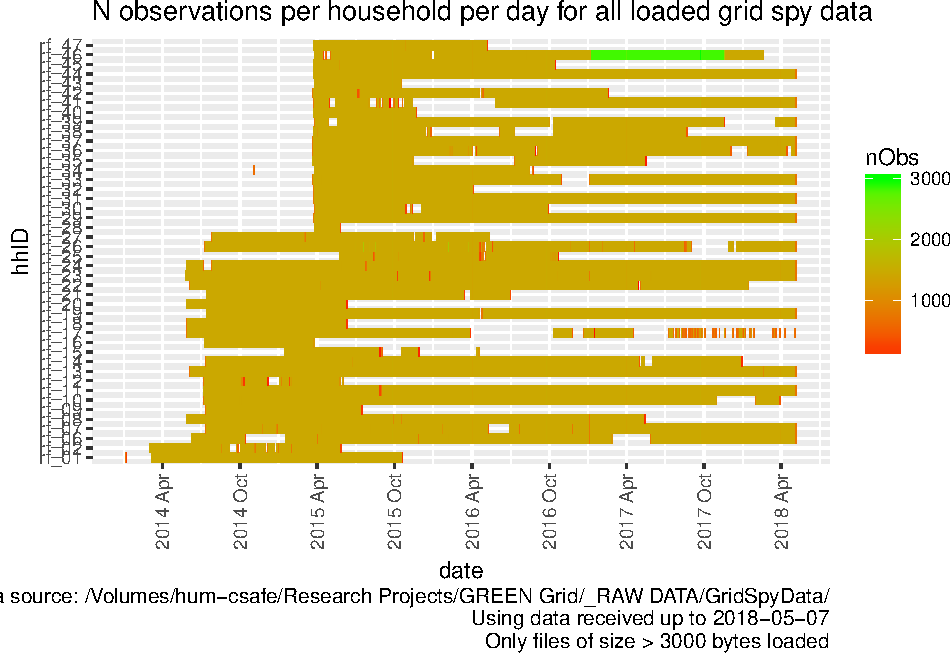
\includegraphics{processNZGGElecCons1minData_files/figure-latex/loadedFilesObsPlots-1.pdf}

\begin{Shaded}
\begin{Highlighting}[]
\KeywordTok{ggsave}\NormalTok{(}\KeywordTok{paste0}\NormalTok{(outPath, }\StringTok{"gridSpyLoadedFileNobsTilePlot.png"}\NormalTok{))}
\end{Highlighting}
\end{Shaded}

\begin{verbatim}
## Saving 6.5 x 4.5 in image
\end{verbatim}

\begin{Shaded}
\begin{Highlighting}[]
\CommentTok{# point plot ----}
\KeywordTok{ggplot}\NormalTok{(hhStatDT, }\KeywordTok{aes}\NormalTok{( }\DataTypeTok{x =}\NormalTok{ date, }\DataTypeTok{y =}\NormalTok{ nObs, }\DataTypeTok{colour =}\NormalTok{ hhID)) }\OperatorTok{+}
\StringTok{  }\KeywordTok{geom_point}\NormalTok{() }\OperatorTok{+}
\StringTok{  }\KeywordTok{scale_x_date}\NormalTok{(}\DataTypeTok{date_labels =} \StringTok{"%Y %b"}\NormalTok{, }\DataTypeTok{date_breaks =} \StringTok{"6 months"}\NormalTok{) }\OperatorTok{+}
\StringTok{  }\KeywordTok{theme}\NormalTok{(}\DataTypeTok{axis.text.x =} \KeywordTok{element_text}\NormalTok{(}\DataTypeTok{angle =} \DecValTok{90}\NormalTok{, }\DataTypeTok{vjust =} \FloatTok{0.5}\NormalTok{, }\DataTypeTok{hjust =} \FloatTok{0.5}\NormalTok{)) }\OperatorTok{+}\StringTok{ }
\StringTok{  }\KeywordTok{labs}\NormalTok{(}\DataTypeTok{title =} \StringTok{"N observations per household per day for all loaded grid spy data"}\NormalTok{,}
       \DataTypeTok{caption =} \KeywordTok{paste0}\NormalTok{(myCaption,}
                        \StringTok{"}\CharTok{\textbackslash{}n}\StringTok{Only files of size > "}\NormalTok{, dataThreshold, }\StringTok{" bytes loaded"}\NormalTok{)}
       
\NormalTok{  )}
\end{Highlighting}
\end{Shaded}

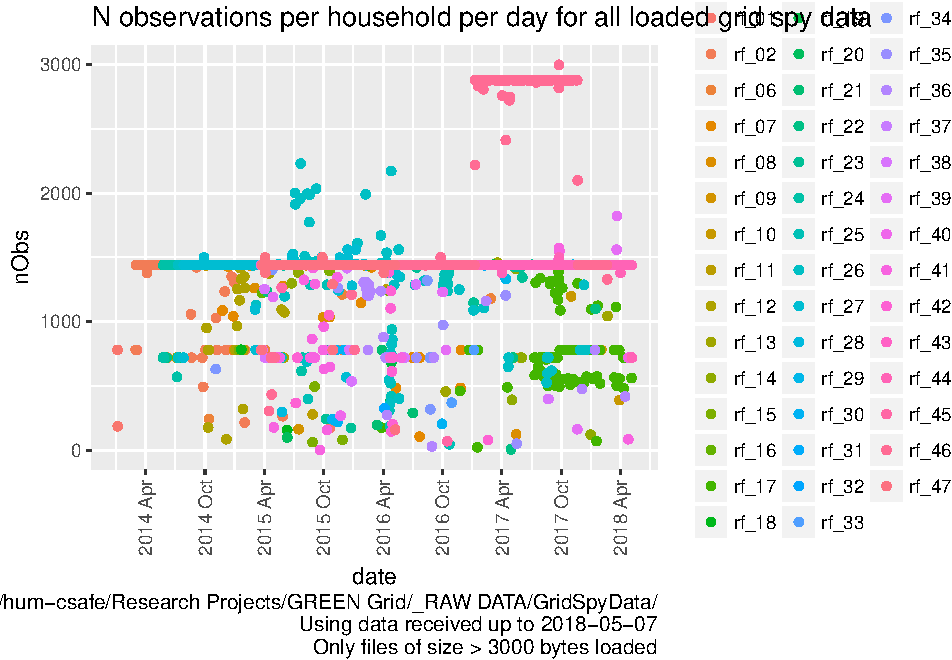
\includegraphics{processNZGGElecCons1minData_files/figure-latex/loadedFilesObsPlots-2.pdf}

\begin{Shaded}
\begin{Highlighting}[]
\KeywordTok{ggsave}\NormalTok{(}\KeywordTok{paste0}\NormalTok{(outPath, }\StringTok{"gridSpyLoadedFileNobsPointPlot.png"}\NormalTok{))}
\end{Highlighting}
\end{Shaded}

\begin{verbatim}
## Saving 6.5 x 4.5 in image
\end{verbatim}

The following table shows the min/max observations per day and min/max
dates for each household. As above, we should not see:

\begin{itemize}
\tightlist
\item
  dates before 2014 or in to the future (indicates date conversion
  errors)
\item
  more than 1440 observations per day (indicates potentially duplicate
  observations)
\item
  non-integer counts of circuits as it suggests some column errors
\end{itemize}

We should also not see NA in any row (indicates date conversion errors).

If we do see any of these then we still have data cleaning work to do!

\begin{Shaded}
\begin{Highlighting}[]
\CommentTok{# Stats table (so we can pick out the dateTime errors)}
\NormalTok{t <-}\StringTok{ }\NormalTok{hhStatDT[, .(}\DataTypeTok{minObs =} \KeywordTok{min}\NormalTok{(nObs),}
             \DataTypeTok{maxObs =} \KeywordTok{max}\NormalTok{(nObs), }\CommentTok{# should not be more than 1440, if so suggests duplicates}
             \DataTypeTok{meanNDataColumns =}\KeywordTok{mean}\NormalTok{(nDataColumns), }\CommentTok{#i.e. n circuits}
             \DataTypeTok{minDate =} \KeywordTok{min}\NormalTok{(date),}
             \DataTypeTok{maxDate =} \KeywordTok{max}\NormalTok{(date)),}
\NormalTok{         keyby =}\StringTok{ }\NormalTok{.(hhID)]}

\KeywordTok{kable}\NormalTok{(}\DataTypeTok{caption =} \StringTok{"Summary observation stats by hhID"}\NormalTok{, t)}
\end{Highlighting}
\end{Shaded}

\begin{longtable}[]{@{}lrrrll@{}}
\caption{Summary observation stats by hhID}\tabularnewline
\toprule
hhID & minObs & maxObs & meanNDataColumns & minDate &
maxDate\tabularnewline
\midrule
\endfirsthead
\toprule
hhID & minObs & maxObs & meanNDataColumns & minDate &
maxDate\tabularnewline
\midrule
\endhead
rf\_01 & 171 & 1500 & 6 & 2014-01-05 & 2015-10-20\tabularnewline
rf\_02 & 215 & 1440 & 6 & 2014-03-02 & 2015-05-28\tabularnewline
rf\_06 & 243 & 1500 & 6 & 2014-06-08 & 2018-05-06\tabularnewline
rf\_07 & 105 & 1500 & 6 & 2014-07-13 & 2018-05-06\tabularnewline
rf\_08 & 123 & 1500 & 6 & 2014-05-28 & 2017-05-15\tabularnewline
rf\_09 & 163 & 1500 & 6 & 2014-07-13 & 2015-07-16\tabularnewline
rf\_10 & 389 & 1500 & 6 & 2014-07-08 & 2018-03-29\tabularnewline
rf\_11 & 278 & 1500 & 6 & 2014-07-07 & 2018-05-06\tabularnewline
rf\_12 & 85 & 1500 & 6 & 2014-07-08 & 2015-06-02\tabularnewline
rf\_13 & 456 & 1500 & 6 & 2014-06-05 & 2018-05-06\tabularnewline
rf\_14 & 120 & 1500 & 6 & 2014-07-13 & 2017-12-30\tabularnewline
rf\_15 & 62 & 1440 & 6 & 2015-01-14 & 2016-04-18\tabularnewline
rf\_16 & 720 & 1500 & 6 & 2014-07-09 & 2015-03-25\tabularnewline
rf\_17 & 22 & 1500 & 6 & 2014-05-29 & 2018-05-05\tabularnewline
rf\_18 & 157 & 1500 & 6 & 2014-05-29 & 2015-06-11\tabularnewline
rf\_19 & 387 & 1500 & 9 & 2014-07-14 & 2018-05-06\tabularnewline
rf\_20 & 98 & 1500 & 6 & 2014-05-28 & 2015-06-11\tabularnewline
rf\_21 & 195 & 1500 & 6 & 2014-07-14 & 2016-07-01\tabularnewline
rf\_22 & 6 & 1500 & 6 & 2014-06-05 & 2018-01-14\tabularnewline
rf\_23 & 171 & 1500 & 6 & 2014-05-25 & 2018-05-06\tabularnewline
rf\_24 & 571 & 1500 & 6 & 2014-05-28 & 2018-05-06\tabularnewline
rf\_25 & 45 & 1500 & 6 & 2015-05-24 & 2016-10-22\tabularnewline
rf\_26 & 362 & 2231 & 6 & 2014-07-10 & 2018-05-06\tabularnewline
rf\_27 & 567 & 1560 & 6 & 2014-07-27 & 2016-05-13\tabularnewline
rf\_28 & 297 & 1440 & 6 & 2015-03-26 & 2015-05-26\tabularnewline
rf\_29 & 720 & 1500 & 6 & 2015-03-25 & 2018-05-06\tabularnewline
rf\_30 & 205 & 1500 & 6 & 2015-03-27 & 2016-09-29\tabularnewline
rf\_31 & 720 & 1500 & 6 & 2015-03-25 & 2018-05-06\tabularnewline
rf\_32 & 325 & 1500 & 6 & 2015-03-25 & 2016-04-05\tabularnewline
rf\_33 & 369 & 1500 & 6 & 2015-03-23 & 2018-05-06\tabularnewline
rf\_34 & 317 & 1500 & 6 & 2014-11-03 & 2016-08-24\tabularnewline
rf\_35 & 50 & 1500 & 6 & 2015-03-22 & 2017-05-17\tabularnewline
rf\_36 & 29 & 1500 & 6 & 2015-03-23 & 2018-05-06\tabularnewline
rf\_37 & 720 & 1500 & 6 & 2015-03-23 & 2018-05-06\tabularnewline
rf\_38 & 398 & 1500 & 6 & 2015-03-24 & 2017-08-22\tabularnewline
rf\_39 & 163 & 1823 & 5 & 2015-03-27 & 2018-05-06\tabularnewline
rf\_40 & 268 & 1500 & 6 & 2015-03-24 & 2015-11-22\tabularnewline
rf\_41 & 1 & 1573 & 6 & 2015-03-25 & 2018-05-06\tabularnewline
rf\_42 & 79 & 1500 & 6 & 2015-03-23 & 2017-02-18\tabularnewline
rf\_43 & 780 & 1495 & 6 & 2015-03-26 & 2015-10-18\tabularnewline
rf\_44 & 720 & 1500 & 6 & 2015-03-24 & 2018-05-06\tabularnewline
rf\_45 & 69 & 1499 & 6 & 2015-03-24 & 2016-10-15\tabularnewline
rf\_46 & 305 & 3000 & 13 & 2015-03-26 & 2018-02-19\tabularnewline
rf\_47 & 159 & 1500 & 6 & 2015-03-24 & 2016-05-08\tabularnewline
\bottomrule
\end{longtable}

Finally we show the total number of households which we think are still
sending data.

\begin{Shaded}
\begin{Highlighting}[]
\NormalTok{plotDT <-}\StringTok{ }\NormalTok{hhStatDT[, .(}\DataTypeTok{nHH =} \KeywordTok{uniqueN}\NormalTok{(hhID)), keyby =}\StringTok{ }\NormalTok{.(date)]}

\CommentTok{# point plot ----}
\KeywordTok{ggplot}\NormalTok{(plotDT, }\KeywordTok{aes}\NormalTok{( }\DataTypeTok{x =}\NormalTok{ date, }\DataTypeTok{y =}\NormalTok{ nHH)) }\OperatorTok{+}
\StringTok{  }\KeywordTok{geom_point}\NormalTok{() }\OperatorTok{+}
\StringTok{  }\KeywordTok{scale_x_date}\NormalTok{(}\DataTypeTok{date_labels =} \StringTok{"%Y %b"}\NormalTok{, }\DataTypeTok{date_breaks =} \StringTok{"6 months"}\NormalTok{) }\OperatorTok{+}
\StringTok{  }\KeywordTok{theme}\NormalTok{(}\DataTypeTok{axis.text.x =} \KeywordTok{element_text}\NormalTok{(}\DataTypeTok{angle =} \DecValTok{90}\NormalTok{, }\DataTypeTok{vjust =} \FloatTok{0.5}\NormalTok{, }\DataTypeTok{hjust =} \FloatTok{0.5}\NormalTok{)) }\OperatorTok{+}\StringTok{ }
\StringTok{  }\KeywordTok{labs}\NormalTok{(}\DataTypeTok{title =} \StringTok{"N live households per day for all loaded grid spy data"}\NormalTok{,}
       \DataTypeTok{caption =} \KeywordTok{paste0}\NormalTok{(myCaption,}
                        \StringTok{"}\CharTok{\textbackslash{}n}\StringTok{Only files of size > "}\NormalTok{, dataThreshold, }\StringTok{" bytes loaded"}\NormalTok{)}
       
\NormalTok{  )}
\end{Highlighting}
\end{Shaded}

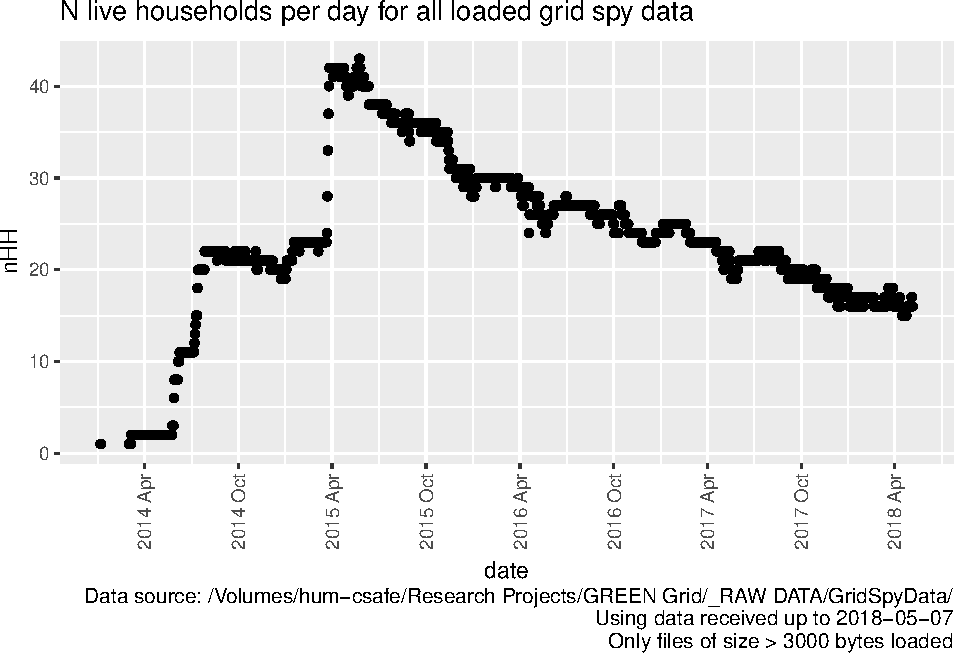
\includegraphics{processNZGGElecCons1minData_files/figure-latex/liveDataHouseholds-1.pdf}

\begin{Shaded}
\begin{Highlighting}[]
\KeywordTok{ggsave}\NormalTok{(}\KeywordTok{paste0}\NormalTok{(outPath, }\StringTok{"gridSpyLiveHouseholdsToDate.png"}\NormalTok{))}
\end{Highlighting}
\end{Shaded}

\begin{verbatim}
## Saving 6.5 x 4.5 in image
\end{verbatim}

\section{Runtime}\label{runtime}

\begin{Shaded}
\begin{Highlighting}[]
\NormalTok{t <-}\StringTok{ }\KeywordTok{proc.time}\NormalTok{() }\OperatorTok{-}\StringTok{ }\NormalTok{startTime}

\NormalTok{elapsed <-}\StringTok{ }\NormalTok{t[[}\DecValTok{3}\NormalTok{]]}
\end{Highlighting}
\end{Shaded}

Analysis completed in 1.3165859\times 10\^{}\{4\} seconds ( 219.43
minutes) using \href{https://cran.r-project.org/package=knitr}{knitr} in
\href{http://www.rstudio.com}{RStudio} with R version 3.4.4 (2018-03-15)
running on x86\_64-apple-darwin15.6.0.

\section{R environment}\label{r-environment}

R packages used: data.table, lubridate, ggplot2, readr, dplyr, knitr

\begin{itemize}
\tightlist
\item
  base R - for the basics (R Core Team 2016)
\item
  data.table - for fast (big) data handling (Dowle et al. 2015)
\item
  lubridate - date manipulation (Grolemund and Wickham 2011)
\item
  ggplot2 - for slick graphics (Wickham 2009)
\item
  readr - for csv reading/writing (Wickham, Hester, and Francois 2016)
\item
  dplyr - for select and contains (Wickham and Francois 2016)
\item
  knitr - to create this document (Xie 2016)
\item
  greenGridr - for local NZ GREEN Grid utilities
\end{itemize}

\begin{Shaded}
\begin{Highlighting}[]
\KeywordTok{sessionInfo}\NormalTok{()}
\end{Highlighting}
\end{Shaded}

\begin{verbatim}
## R version 3.4.4 (2018-03-15)
## Platform: x86_64-apple-darwin15.6.0 (64-bit)
## Running under: macOS High Sierra 10.13.4
## 
## Matrix products: default
## BLAS: /Library/Frameworks/R.framework/Versions/3.4/Resources/lib/libRblas.0.dylib
## LAPACK: /Library/Frameworks/R.framework/Versions/3.4/Resources/lib/libRlapack.dylib
## 
## locale:
## [1] en_GB.UTF-8/en_GB.UTF-8/en_GB.UTF-8/C/en_GB.UTF-8/en_GB.UTF-8
## 
## attached base packages:
## [1] stats     graphics  grDevices utils     datasets  methods   base     
## 
## other attached packages:
## [1] knitr_1.20          dplyr_0.7.4         readr_1.1.1        
## [4] ggplot2_2.2.1       lubridate_1.7.4     data.table_1.10.4-3
## [7] greenGridr_0.1.0   
## 
## loaded via a namespace (and not attached):
##  [1] Rcpp_0.12.16      bindr_0.1.1       magrittr_1.5     
##  [4] hms_0.4.2         munsell_0.4.3     colorspace_1.3-2 
##  [7] R6_2.2.2          rlang_0.2.0.9001  highr_0.6        
## [10] stringr_1.3.0     plyr_1.8.4        tools_3.4.4      
## [13] grid_3.4.4        gtable_0.2.0      htmltools_0.3.6  
## [16] assertthat_0.2.0  yaml_2.1.18       lazyeval_0.2.1   
## [19] rprojroot_1.3-2   digest_0.6.15     tibble_1.4.2     
## [22] bindrcpp_0.2.2    glue_1.2.0        evaluate_0.10.1  
## [25] rmarkdown_1.9     labeling_0.3      stringi_1.1.7    
## [28] compiler_3.4.4    pillar_1.2.2      scales_0.5.0.9000
## [31] backports_1.1.2   pkgconfig_2.0.1
\end{verbatim}

\hypertarget{refs}{}
\hypertarget{ref-data.table}{}
Dowle, M, A Srinivasan, T Short, S Lianoglou with contributions from R
Saporta, and E Antonyan. 2015. \emph{Data.table: Extension of
Data.frame}. \url{https://CRAN.R-project.org/package=data.table}.

\hypertarget{ref-lubridate}{}
Grolemund, Garrett, and Hadley Wickham. 2011. ``Dates and Times Made
Easy with lubridate.'' \emph{Journal of Statistical Software} 40 (3):
1--25. \url{http://www.jstatsoft.org/v40/i03/}.

\hypertarget{ref-baseR}{}
R Core Team. 2016. \emph{R: A Language and Environment for Statistical
Computing}. Vienna, Austria: R Foundation for Statistical Computing.
\url{https://www.R-project.org/}.

\hypertarget{ref-ggplot2}{}
Wickham, Hadley. 2009. \emph{Ggplot2: Elegant Graphics for Data
Analysis}. Springer-Verlag New York. \url{http://ggplot2.org}.

\hypertarget{ref-dplyr}{}
Wickham, Hadley, and Romain Francois. 2016. \emph{Dplyr: A Grammar of
Data Manipulation}. \url{https://CRAN.R-project.org/package=dplyr}.

\hypertarget{ref-readr}{}
Wickham, Hadley, Jim Hester, and Romain Francois. 2016. \emph{Readr:
Read Tabular Data}. \url{https://CRAN.R-project.org/package=readr}.

\hypertarget{ref-knitr}{}
Xie, Yihui. 2016. \emph{Knitr: A General-Purpose Package for Dynamic
Report Generation in R}. \url{https://CRAN.R-project.org/package=knitr}.


\end{document}
